
\chapter*{ಅನುಬಂಧ : (1)}

\section*{ಮಾಯಾಚೌಕದ ಇತಿಹಾಸ :}

ಮಾಯಾಚೌಕದ ಉಗಮ ಹಾಗೂ ಇತಿಹಾಸ ಮಸಕಾಗಿದೆ. ಅಲ್ಲದೇ ನಿಗೂಢವೂ ಆಗಿದೆ. ಶಾಸ್ತ್ರ-ಜಿಜ್ಞಾಸುಗಳಿಂದ ಸಮರ್ಪಕ ಸಂಶೋಧನೆಗಳು ನಡೆದಿಲ್ಲದಿರುವುದು ಇದಕ್ಕೆ ಒಂದು \linebreak ಕಾರಣ. ಪರಿಣಾಮವಾಗಿ ಮಾಯಾಚೌಕಗಳ ಉಗಮದ ಬಗ್ಗೆ ತಿಳಿದಿರುವ ವಿಷಯಗಳು \linebreak ಪರಸ್ಪರ ವಿರೋಧವಾಗಿವೆ. ಕೆಲವೊಮ್ಮೆ ಉತ್ಪ್ರೇಕ್ಷೆಗೆ ಗುರಿಯಾಗಿವೆ. ಕ್ರಿ.ಶ. 1300ಕ್ಕೆ ಹಿಂದಿನ ಕಾಲದ ಮಾಯಾಚೌಕಗಳ ಇತಿಹಾಸದ ಬಗ್ಗೆ ಲಭಿಸಿರುವ ವಿವರಗಳು ಅತಿ ಕಡಿಮೆ.

ಒಂದು ಚಚ್ಚೌಕವನ್ನು ಅಡ್ಡಲಾಗಿ ಮತ್ತು ಉದ್ದವಾಗಿ ಸಮಾನ ಸಂಖ್ಯೆಯ ಸರಳ ರೇಖೆಗಳಿಂದ ವಿಭಾಗಿಸಿ. ಚಿಕ್ಕ ಚಿಕ್ಕ ಮನೆಗಳಿರುವ ಹಂದರ ಲಭಿಸುತ್ತದೆ. ಈ ಮನೆಗಳಲ್ಲಿ ಸಂಖ್ಯೆಗಳನ್ನೋ, ಅಕ್ಷರಗಳನ್ನೋ, ತುಂಬಿಸಿದಾಗ ಅಂತಹ ಚೌಕಗಳಿಗೆ ವಿಶೇಷ ಗುಣಗಳಿರು\-ವುದಾಗಿ ನಂಬಲಾಗಿತ್ತು. ಹಾಗಾಗಿ ಇಂತಹ ಚೌಕಗಳಿಗೆ ಮಾಯಾಚೌಕಗಳೆಂಬ ಹೆಸರು ಬಂದಿತು. \linebreak ಪ್ರಾರಂಭದ ದಿನಗಳಲ್ಲಿ ಮಾಯಾಚೌಕಗಳನ್ನು ಧಾರ್ಮಿಕ ಚಿಹ್ನೆಗಳಾಗಿ ಬಳಸಿದರೂ ನಂತ\-ರದ ದಿನಗಳಲ್ಲಿ ಅವು ರಕ್ಷಾ ತಾಯಿತಗಳಾದವು. ಇವುಗಳನ್ನು ಭೂತಪ್ರೇತಗಳಿಂದ ರಕ್ಷಣೆ ಒದಗಿಸುವ ತಡೆಗಳೆಂದೂ, ರೋಗ ನಿವಾರಕ ಅಸ್ತ್ರಗಳೆಂದೂ, ಕಾಲ ಜ್ಞಾನ ಸೂಚಕಗಳೆಂದೂ ಬಳಸ\-ಲಾಯಿತು. ಕಾಲಕ್ರಮೇಣ ಇವುಗಳ ಪ್ರಭಾವದ ಬಗ್ಗೆ ಭ್ರಮೆ ನಿರಸನವಾಗಿ ಇವು ಕೇವಲ ಕುತೂ\-ಹಲಕಾರಿಗಳಾಗಿ ಹಾಗೂ ಒಗಟಾಗಿ ಉಳಿದುವು. ಬೆರಳೆಣಿಕೆಯಷ್ಟು ಗಣಿತಜ್ಞರು  \hbox{ಮಾತ್ರ} ಇವುಗಳನ್ನು ಸಂಖ್ಯಾಲೋಕದಲ್ಲಿ ಅಧ್ಯಯನ ಮಾಡಿದ್ದುಂಟು.

ಪಾಶ್ಚಾತ್ಯ ಜಗತ್ತಿನಲ್ಲಿ ಅತಿಪ್ರಸಿದ್ಧವಾಗಿದ್ದ ಅಕ್ಷರ ಚೌಕವೆಂದರೆ, SATOR ಚೌಕ. ಇದರಲ್ಲಿನ ಪದಗಳು SATOR, AREPO, TENET, OPERA ಮತ್ತು ROTAS. ಈ ಪದಗಳು ಅರ್ಥರಹಿತವೆಂದು ಕಂಡುಬಂದರೂ ಕೆಲವರು ಹೀಗೆ ಅರ್ಥೈಸಿದ್ದಾರೆ. ‘‘Farmer Arepo stears the Plough’’ ‘‘The Farmer Arepo keeps the world rolling.’’

ಮಧ್ಯದಲ್ಲಿ ಒಂದು ಶಿಲುಬೆ ಆಕೃತಿ ಉಂಟಾಗುತ್ತದೆ. (ಚಿತ್ರದಲ್ಲಿ ಕಪ್ಪು ಮಾಡಿದೆ)
\begin{figure}[H]
\includegraphics[scale=.9]{src/figures/chap9/fig9-1.eps}
\end{figure}

ಈ ಚೌಕದ ಮಾದರಿಗಳು ಪಾಂಪೆ ನಗರದ ಅವಶೇಷಗಳಲ್ಲಿ ದೊರೆತಿವೆ. ಇವನ್ನು ಕ್ರಿ.ಶ. 1ನೆಯ ಶತಮಾನಕ್ಕೆ ಸೇರಿದವೆಂದು ಹೇಳಲಾಗಿದೆ. ಅಷ್ಟೇ ಅಲ್ಲದೇ 19ನೆಯ ಶತಮಾನದಲ್ಲಿ ಸಹ ಇವುಗಳಿಂದ ಬೆಂಕಿ, ತುಡುಗು, ಅನಾರೋಗ್ಯ ಮತ್ತಿತರ ಅವಘಡಗಳಿಂದ ರಕ್ಷಣೆ ಪಡೆಯ ಬಹುದೆಂದು ನಂಬಲಾಗಿತ್ತು. ಭಾರತದಲ್ಲಿಯೂ ಸಹ ಧಾರ್ಮಿಕ ಕ್ರಿಯೆಗಳಿಗೆ ಮಾಯಾ\-ಚೌಕಗಳನ್ನು ಬಳಸುತ್ತಿದ್ದುದುಂಟು. ಮಾನದೇವ ಸೂರಿ ಎಂಬ ಜೈನ ಗಣಿತಜ್ಞನು 16ಮನೆಗಳ ಮಾಯಾ\-ಚೌಕವನ್ನು ಬೀಜ ಯಂತ್ರವಾಗಿ ಬಳಸುವುದನ್ನು ತನ್ನ ಲಘು ಶಾಂತಿಸ್ತೋತ್ರದಲ್ಲಿ ಸೂಚಿಸಿ\-ದ್ದಾನೆ. ಶುಭಸುಂದರ ಎಂಬ ಗಣಿತಜ್ಞನು 16 ಮನೆಗಳ ಮಾಯಾಚೌಕವನ್ನು ಬೀಜಯಂತ್ರವಾಗಿ ಬಳಸುವುದನ್ನು ತನ್ನ ಯುಗಾದಿ ದೇವ ಸ್ತೋತ್ರದಲ್ಲಿ 25 ಮತ್ತು 64 ಮನೆಗಳ ಚೌಕಗಳನ್ನು ಕೊಟ್ಟಿರುವುದು ತಿಳಿದು ಬಂದಿದೆ. ಕ್ರಿ.ಶ. 1356ರಲ್ಲಿ ನಾರಾಯಣಪಂಡಿತನು ರಚಿಸಿದ ‘‘ಗಣಿತ ಕೌಮುದಿ’’ ಎಂಬ ಸಂಸ್ಕತ ಗ್ರಂಥದಲ್ಲಿ ಮಾಯಾಚೌಕ, ಮಾಯಾವೃತ್ತಗಳ ಬೇರೆ ಬೇರೆ ಮಾದರಿಗಳನ್ನು ಕೊಟ್ಟಿದ್ದಾನೆ.

ಅರಬ್ಬರು ಮತ್ತು ಯಹೂದಿಗಳು ದೈವಧ್ಯಾನಕ್ಕಾಗಿ ಬಳಸುತ್ತಿದ್ದ ಪವಿತ್ರ ನಾಮಗಳೂ, ಪದಗುಚ್ಛಗಳೂ, ಕೆಲವು ಚೌಕಗಳಲ್ಲಿ ಕಂಡುಬಂದಿವೆ. ಇಷ್ಟು ಮಾತ್ರವಲ್ಲ. ಸಂಖ್ಯಾ ಚೌಕಗಳೂ ಗಣನೀಯ ಪ್ರಮಾಣದಲ್ಲಿ ಬಳಕೆ ಆಗುತ್ತಿದ್ದುದಕ್ಕೆ ಪುರಾವೆಗಳು ದೊರೆತಿವೆ.

ಸಂಖ್ಯೆಗಳನ್ನೊಳಗೊಂಡ ಚೌಕಗಳು ಮಾಯಾಚೌಕಗಳೆನಿಸಿದ್ದು ಅವುಗಳ ವಿಶಿಷ್ಟ ಲಕ್ಷಣ ಗಳಿಗಾಗಿ. ಕೆಲವು ಸಂಖ್ಯೆಗಳು ಮಾನವರಿಗೆ ಒಳಿತು ಅಥವಾ ಕೆಡಕನ್ನುಂಟುಮಾಡುವುವೆಂದು ಭಾವಿಸಿ ಅವುಗಳ ಬಗ್ಗೆ ಭಯಮಿಶ್ರಿತ ಭಾವನೆಯನ್ನು ಸೂಚಿಸುವ ಸಂಖ್ಯಾ ಜ್ಯೋತಿಷ್ಯಕ್ಕೂ ಮಾಯಾಚೌಕಕ್ಕೂ ಯಾವ ಸಂಬಂಧವೂ ಇಲ್ಲ. ಕಾಲಕ್ರಮೇಣ ನಂಬಿಕೆಗಳು ಬದಲಾದರೂ ಸಂಖ್ಯಾ\-ಚೌಕಗಳನ್ನು ಪವಿತ್ರ ಚಿಹ್ನೆಯಾಗಿಯೋ, ರಕ್ಷಾ ತಾಯಿತವಾಗಿಯೋ ಬಳಸುವುದು ಅಲ್ಲಲ್ಲಿ ಉಳಿದುಕೊಂಡೇ ಬಂದಿತು.

ಮಾಯಾಚೌಕದ ಇತಿಹಾಸದ ಕಡೆ ಕಣ್ಣು ಹಾಯಿಸಿದರೆ ಚೀನಾ, ಭಾರತ ಮತ್ತು ಮಧ್ಯಪ್ರಾಚ್ಯ (ಅರಬ್) ರಾಷ್ಟ್ರಗಳಲ್ಲಿ ಪ್ರಾಚೀನ ಕಾಲದಲ್ಲಿಯೇ ಮಾಯಾ ಚೌಕಗಳ ಬಳಕೆ ಇದ್ದುದು ತಿಳಿದು ಬರುತ್ತದೆ. ಇವುಗಳ ವಿವರ ಹೀಗಿದೆ.

\section*{ಚೀನಾ :}

ಕ್ರಿ.ಪೂ. 4ನೆಯ ಶತಮಾನದ ಕೆಲವು ದಾಖಲೆಗಳಲ್ಲಿ 9 ಮನೆಯ ($3 \times 3$) ಮಾಯಾಚೌಕಗಳು ಇದ್ದುವೆಂದು ತಿಳಿದುಬಂದಿದೆ. ಜಗತ್ತಿನ ಇತರ ಭಾಗಗಳಲ್ಲಿ ಹಲವು ಶತಮಾನಗಳ ನಂತರದ\-ವರೆಗೂ ಇವು ಕಂಡುಬಂದಿಲ್ಲ. ಒಂದು ದಂತ ಕತೆಯನ್ವಯ ಯಾರೋ ಒಬ್ಬ ಅಜ್ಞಾತ ಗಣಿತಜ್ಞನು ನದಿಯಿಂದ ಹೊರಬಂದ ಆಮೆಯ ಬೆನ್ನಿನ ಮೇಲೆ 9 ಮನೆಯ ಚೌಕವನ್ನು ಕಂಡನಂತೆ. ಈ ಚೌಕಕ್ಕೆ \textbf{‘‘ಲೋಷೂ’’} ಚೌಕವೆಂದು ಹೆಸರಿಡಲಾಗಿದೆ. \textbf{‘‘ಲೋಷೂ’’} ಎಂದರೆ ನದಿ ನಕ್ಷೆ. ನದಿ ದೇವತೆಗೆ ನೀಡಬೇಕಾದ ಧಾರ್ಮಿಕ ಬಲಿಯ ಸಂಬಂಧದಲ್ಲಿ ಈ ಆಮೆ ಕಾಣಿಸಿಕೊಂಡಿತೆಂದು ಪ್ರತೀತಿ. ಹಿಂದಿನ ಕಾಲದಿಂದಲೂ ಗಣಿತದ ರಚನೆಗಳು ಅಲೌಕಿಕ ಅಂಶಗಳ ಜೊತೆಗೆ ತಳುಕಾಗಿರುವುದನ್ನು ಕಾಣುತ್ತೇವೆ.

\smallskip
ಇವಿಷ್ಟೇ ಅಲ್ಲದೇ ಲೋಷೂ ರಚನೆಯನ್ನು ಮಿಂಗ್ ಟಾಂಗ್ ಎಂಬ ಪೌರಾಣಿಕ ರಾಜನ ಅರಮನೆಯ ಭೂ ವಿನ್ಯಾಸಕ್ಕೆ ಹೊಂದಿಸಿದರು ಕೆಲವರು. ಆದರೆ ಅರಮನೆಯ ವಿನ್ಯಾಸಕ್ಕೂ ಲೋಷೂ ಚೌಕಕ್ಕೂ ಸಂಬಂಧ ಹೇಗೆ? ಇದರ ಬಗ್ಗೆ ಎಲ್ಲೂ ವಿವರಗಳಿಲ್ಲ. ಇಷ್ಟು ಮಾತ್ರವಲ್ಲದೆ ಲೋಷೂ ಚೌಕಕ್ಕೂ ಇ-ಚಾಂಗ್ ಎಂಬ ರಾಜನಿಗೂ ಸಂಬಂಧ ಕಲ್ಪಿಸಲಾಗಿದೆ. \hbox{ಇದಕ್ಕೂ} ಯಾವ ಪುರಾವೆಗಳೂ ದೊರೆತಿಲ್ಲ. ಲೊಷೂ ಚೌಕದ ಕುರಿತು ಅತಿ ಪುರಾತನ ದಾಖಲೆಗಳು ಸಂದಿಗ್ಧಾರ್ಥವಾದರೂ ಕ್ರಿ.ಪೂ. 650ರ ಸುಮಾರಿನ ಷು ಚಿಂಗ್ ಎಂಬಾತನ ಬಗೆಗೆ ದೊರೆತ ಮಾಹಿತಿಯಲ್ಲಿ, ಅವನು ನದಿ ನಕ್ಷೆ ಬರೆದುದಾಗಿಯೂ ಅದು $3 \times 3$ ರ ಮಾಯಾಚೌಕ \hbox{ವಿರಬಹುದೆಂದೂ} ತಿಳಿದು ಬಂದಿದೆ. ಕ್ರಿ.ಪೂ.500ರಿಂದ 300ರಲ್ಲಿ ಯೂ ನದಿ ನಕ್ಷೆಯ \hbox{ಕುರಿತು} ಉಲ್ಲೇಖವಿದ್ದರೂ ಯಾವುದೇ ನಿರ್ದಿಷ್ಟ ಮಾಯಾಚೌಕದ ಮಾಹಿತಿ ದೊರೆತಿಲ್ಲ. ಪ್ರಥಮ ಬಾರಿಗೆ $3 \times 3$ ರ ಮಾಯಾ\-ಚೌಕದ ವಿವರ ಲಭ್ಯವಾಗಿರುವುದು ಕ್ರಿ.ಶ. 80ರಲ್ಲಿದ್ದ ಟಾ ಟೈ ಲಿಚಿಯ ಬರಹ\-ಗಳಿಂದ. ಆದರೆ ಮಾಯಾಚೌಕ ದೊರೆತಿಲ್ಲ. ಕ್ರಿ.ಶ. 570ರಲ್ಲಿದ್ದ ಷೀ ಜೆನ್ ಎಂಬುವವನು $3 \times 3$ ರ ಮಾಯಾಚೌಕದ ಪೂರ್ಣ ವಿವರಗಳನ್ನು ಕೊಟ್ಟಿದ್ದಾನೆ. ನಂತರ ಕ್ರಿ.ಶ. 1275ರ ವರೆಗೆ ಚೀನಾದಲ್ಲಿ ಮಾಯಾಚೌಕಗಳ ಬಗೆಗೆ ಯಾವುದೇ ಪ್ರಗತಿ ಕಂಡುಬಂದಂತಿಲ್ಲ. \linebreak ಇದಕ್ಕೆ ಕಾರಣ ಬಹುಶಃ ಚೀಣೀಯರು ಲೋಷೂ ಚೌಕವನ್ನು ಲೌಕಿಕಾತೀತವೆಂದು ಪರಿಗಣಿಸಿ, \break ಮಾನವ ಕುತೂಹಲಕ್ಕೆ ಅದನ್ನು ಒಡ್ಡದೇ ಇದ್ದುದು ಇರಬಹುದು.

\smallskip
ಲೋಷೂ ಚೌಕವನ್ನು ರಚಿಸಲು ಅವರು ಅನುಸರಿಸುತ್ತಿದ್ದ ವಿಧಾನ ಸರಳ. ($3 \times 3$) ಅಂದರೆ 9ಮನೆಗಳ ಒಂದು ಚೌಕ ರಚಿಸಿ, ಅದರಲ್ಲಿ ಕ್ರಮವಾಗಿ 1 ರಿಂದ 9 ವರೆಗಿನ ಸಂಖ್ಯೆ ತುಂಬಿಸುತ್ತಿದ್ದರು. (ಚಿತ್ರ. ಅ.1 ನೋಡಿ) ನಂತರ ಈ ಚೌಕವನ್ನು $45^\circ$ಗಳಷ್ಟು ಪ್ರದಕ್ಷಿಣವಾಗಿ ಓರೆ ಮಾಡಿ, (ಚಿತ್ರ ಅ -2 ನೋಡಿ) ಮಧ್ಯದ ಅಡ್ಡಸಾಲು ಮತ್ತು ಕಂಭಸಾಲುಗಳಲ್ಲಿನ ಎದುರು ಬದುರುಸಂಖ್ಯೆಗಳನ್ನು ಅದಲು ಬದಲು ಮಾಡುತ್ತಿದ್ದರು. (ಚಿತ್ರ. ಅ.3 ನೋಡಿ) ಉಂಟಾದ ವಜ್ರಾಕೃತಿಯ ಮೇಲಿನ ಕೆಳಗಿನ ತುದಿಗಳನ್ನು ಒಳಕ್ಕೆ ತಳ್ಳಿ ಚಚ್ಚೌಕ ಪಡೆಯುತ್ತಿದ್ದರು. ಅದು $3 \times 3$ರ ಮಾಯಾಚೌಕವಾಗಿರುತ್ತಿದ್ದಿತು. (ಚಿತ್ರ.ಅ.4 ನೋಡಿ)
\begin{figure}[H]
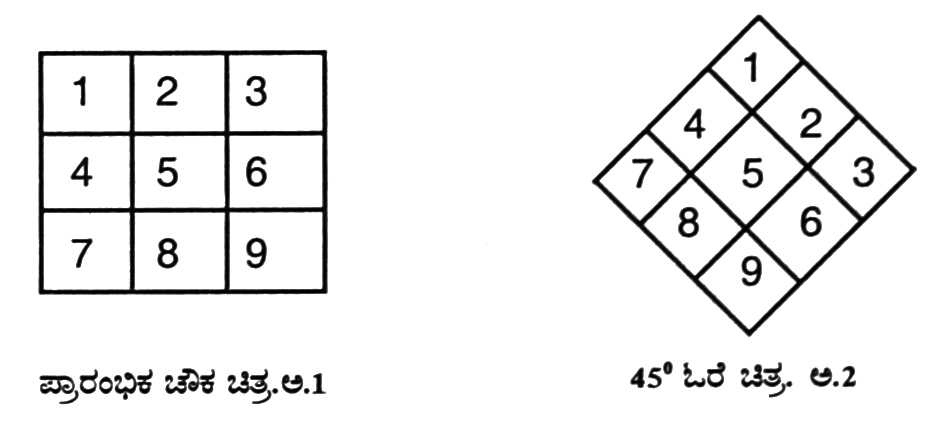
\includegraphics{src/figures/chap9/fig9-2.jpg}
\end{figure}
\begin{figure}[H]
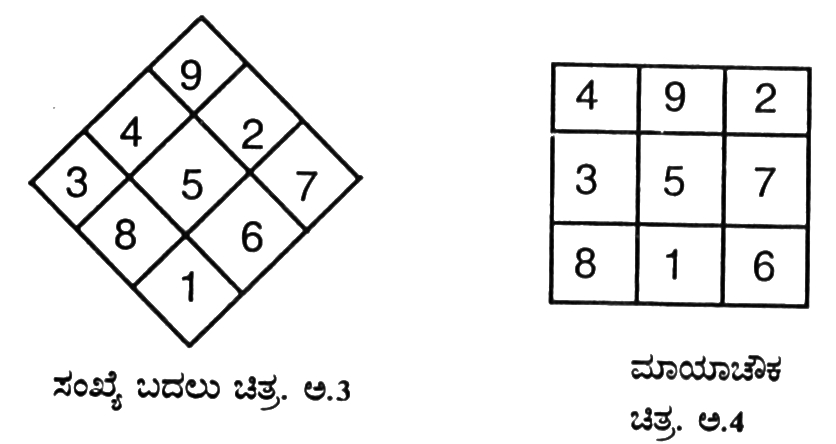
\includegraphics{src/figures/chap9/fig9-3.jpg}
\end{figure}

ಪೌರಾಣಿಕ ಚಕ್ರವರ್ತಿ ಯೂ ಎನ್ನುವವನು ಬಹಳ ಹಿಂದಿನ ಕಾಲದಲ್ಲಿ ಇದನ್ನು ಶೋಧಿಸಿದನೆಂಬ ಪ್ರತೀತಿಯೂ ಇದೆ. ಈ ಚೌಕವು ಚೀನಾ ಸಾಮ್ರಾಜ್ಯವನ್ನು ಪ್ರತಿನಿಧಿಸುವ ಚಿಹ್ನೆ ಎಂದು ನಂಬಲಾಯಿತು. ಹಲವರು ಇದರಲ್ಲಿ ವಿಶಾಲ ವಿಶ್ವವನ್ನು ಗುರುತಿಸಲು ಯತ್ನಿಸಿದರು. ಇದರ ಮಧ್ಯದ ಸಂಖ್ಯೆಯು ಎದುರು ಬದುರು ಸಂಖ್ಯೆಗಳ ಜೋಡಿಗಳಿಗೆ ಕೇಂದ್ರವಾಗಿದ್ದು ಚೀನಾದ ರಾಜನನ್ನು ಪ್ರತಿನಿಧಿಸುತ್ತದೆ ಎಂದು ಕೆಲವರ ಅಭಿಮತ. ಮತ್ತೆ ಕೆಲವರು ಮಧ್ಯದ ಮನೆಯ ಸಂಖ್ಯೆಯು ವಿಶಾಲ ವಿಶ್ವದ ನಡುವಿನ ತಿರುಗು ಅಕ್ಷ ಎಂದು ನಂಬಿದರು. ಈ \linebreak ಚೌಕದ ಕ್ರಮ ಯೋಜನೆ (Permutation) ಯಿಂದ ಲಭಿಸಿದ ಅನೇಕ ಬೇರೆ ಬೇರೆ \linebreak ಚೌಕಗಳನ್ನು ಚೀನಿಯರು ನಂಬಿದ ಪ್ರಾಪಂಚಿಕ ಸತ್ಯಗಳನ್ನು ವಿವರಿಸಲು ಬಳಸಿದರು. ಆ ಚೌಕಗಳಲ್ಲಿ ಯಿನ್ ಮತ್ತು ಯಾಂಗ್ಗಳ ಸಮತೋಲನ, ಪಂಚಭೂತಗಳ ಅನುಕ್ರಮ ಹಾಗೂ ಟಾವೊನ ಕೆಲವು ಸಿದ್ಧಾಂತಗಳು- ಇವುಗಳ ಸಂಕೇತಗಳನ್ನು ಕಾಣಲು ಯತ್ನಿಸಿದರು. ಹೀಗಾಗಿ ಈ ಚೌಕಗಳನ್ನು ಪವಿತ್ರವೇದಿಕೆ ಗಳ ರಚನೆ, ವಿಶ್ವದ ನಕ್ಷೆಯನ್ನು ಬಿಡಿಸುವಿಕೆ ಮತ್ತು ಭವಿಷ್ಯ ಹೇಳಲು ಬಳಸುತ್ತಿದ್ದ ಫಲಕಗಳು ಮೊದಲಾದವುಗಳಲ್ಲಿ ಉಪಯೋಗಿಸತೊಡಗಿದರು.

ಕ್ರಿ.ಶ. 1275ರಲ್ಲಿ ಯಾಂಗ್ ಹುಯೀ ಮಾಯಾಚೌಕಗಳ ಪುಸ್ತಕವನ್ನು ಪ್ರಕಟಿಸಿದ-ನು. ಈ ವೇಳೆಗಾಗಲೇ ಮಾಯಾಚೌಕ ರಚನೆ ಹಳತಾಗಿದ್ದಿತು. ಚೀಣೀಯರು 5 ಮತ್ತು 7 ಕ್ರಮ\-ವರ್ಗಗಳ ಮಾಯಾಚೌಕಗಳನ್ನು ರಚಿಸಲು ಒಂದು ವಿಧಾನವನ್ನು ಕಂಡುಕೊಂಡಿದ್ದರು. ಯಾವ ಕ್ರಮವರ್ಗದ ಮಾಯಾಚೌಕವನ್ನು ರಚಿಸಬೇಕಿತ್ತೋ ಆ ಚೌಕದ ಸಂಖ್ಯೆಗಳ ಅಂಕಗಣಿತ ಶ್ರೇಢಿ\-ಯ (1,2,3,...2) ನಡುವಿನ 9 ಸಂಖ್ಯೆಗಳನ್ನು ಬಳಸಿ 3 ಕ್ರಮವರ್ಗದ ಒಂದು ಮಾಯಾಚೌಕ\-ವನ್ನು ರಚಿಸುತ್ತಿದ್ದರು. ಉಳಿದ ಸಂಖ್ಯೆ ಗಳನ್ನು ಚೌಕದ ಸುತ್ತಾ ಜೊತೆಜೊತೆಯಾಗಿ ಹೊರಗಿನ ಎದುರು ಬದರು ಮನೆಗಳಲ್ಲಿ ತುಂಬಿಸಿ, ಅಡ್ಡಸಾಲು ಹಾಗೂ ಕಂಭಸಾಲುಗಳ ಸಂಖ್ಯೆಗಳ ಮೊತ್ತ ಸಮನಾಗಿರುವಂತೆ ಮಾಡುತ್ತಿದ್ದರು. ಇಷ್ಟೇ ಅಲ್ಲದೆ, ಶ್ರೇಢಿಯ ಮೊದಲ ನಾಲ್ಕು ಸಂಖ್ಯೆಗಳು, ಮಧ್ಯದ ಸಂಖ್ಯೆ ಹಾಗೂ ಕೊನೆಯ ನಾಲ್ಕು ಸಂಖ್ಯೆಗಳು ಒಟ್ಟು 9 ಸಂಖ್ಯೆಗಳನ್ನು ಬಳಸಿ \linebreak ಒಂದು ಲೋಷೂ ಚೌಕ ರಚಿಸಿ, ಉಳಿದ ಸಂಖ್ಯೆಗಳನ್ನೂ ಚೌಕದ ಸುತ್ತಲಿನ ಮನೆಗಳಲ್ಲಿ ತುಂಬಿಸಿ ಮಾಯಾಚೌಕ ಪಡೆಯುವುದನ್ನು ಕಲಿತಿದ್ದರು.

ಲೋಷೂ ಚೌಕದ ಆಧಾರದ ಮೇಲೆ 9 ಕ್ರಮವರ್ಗದ ಮಾಯಾಚೌಕ ರಚಿಸಿರುವುದು \hbox{ವಿಶಿಷ್ಟವಾಗಿದೆ.} ಮೊದಲಿಗೆ 1 ರಿಂದ 81 ರವರೆಗಿನ ಕ್ರಮಾಗತ ಸಂಖ್ಯೆಗಳನ್ನು $9 \times 9$ ಚೌಕ\-ದಲ್ಲಿನ 9 ಕಂಭಸಾಲುಗಳಲ್ಲಿ ಕ್ರಮವಾಗಿ ತುಂಬಿಸುವುದು. (ಚಿತ್ರ. ಅ.5) ನಂತರ ಈ ಚೌಕದ ಪ್ರತಿ ಅಡ್ಡಸಾಲಿನ 9 ಸಂಖ್ಯೆಗಳನ್ನು ಬಳಸಿ 3 ಕ್ರಮವರ್ಗದ ಮಾಯಾಚೌಕ ರಚಿಸುವುದು. ಈ ಒಂಭ\-ತ್ತು $9 \times 9$ ಮಾಯಾಚೌಕಗಳನ್ನು ಅವುಗಳಲ್ಲಿನ ಅತಿ ಚಿಕ್ಕ ಸಂಖ್ಯೆಯನ್ನು \hbox{ಆಧರಿಸಿ ಲೋಷೂ} ಮಾದರಿಯಲ್ಲಿ ಜೋಡಿಸುವುದು. ಅಂದರೆ 1 ಇರುವ ಚೌಕವನ್ನು $3 \times 3$ ಲೋಷೂ ಚೌಕದ 1 ಬರುವ ಸ್ಥಳದಲ್ಲಿ, 2 ಇರುವ ಚೌಕವನ್ನು 2 ರ ಜಾಗದಲ್ಲಿ ಇತ್ಯಾದಿ ಕ್ರಮವಾಗಿ ಜೋಡಿಸಿದರು. $9 \times 9$ರ ಒಂದು ಮಾಯಾಚೌಕ ಸಿದ್ಧವಾಯಿತು. (ಚಿತ್ರ.ಅ. 6. ನೋಡಿ)

(ಅ.6. ಚಿತ್ರದಲ್ಲಿರುವ $9 \times 9$ ಚೌಕದಲ್ಲಿ $3 \times 3$ರ 9 ಚೌಕಗಳಿವೆ. ಇವುಗಳಲ್ಲಿ ರೇಖಾಂಕನ ಮಾಡಿರುವ ಸಂಖ್ಯೆಗಳು ಲೋಷೂ ಚೌಕ ರಚಿಸುತ್ತವೆ. ಆ ಸಂಖ್ಯೆಯಿಂದ ಪ್ರಾರಂಭವಾಗುವ ಅಡ್ಡಸಾಲಿನ 9 ಸಂಖ್ಯೆಗಳು ಆ ಚೌಕದಲ್ಲಿವೆ.)

ಚಿತ್ರ ಅ. 6 ರಲ್ಲಿರುವ ಮಾಯಾಚೌಕದಲ್ಲಿ ಕೇಂದ್ರ ಸಂಖ್ಯೆಯ (41) ಮೂಲಕ ಎಳೆದ ಸರಳರೇಖೆಯ ಮೇಲೆ ಕೇಂದ್ರ ಸಂಖ್ಯೆಯಿಂದ ಸಮಾನ ದೂರದಲ್ಲಿರುವ ಸಂಖ್ಯೆಗಳ ಮೊತ್ತ ಕೇಂದ್ರ ಸಂಖ್ಯೆಯ ಎರಡರಷ್ಟಿರುತ್ತದೆ. ಹಾಗೂ ಕೇಂದ್ರ ಸಂಖ್ಯೆಗೆ ಓರೆ ಸ್ಥಾನ (ಖkಛಿಡಿ) ಗಳಲ್ಲಿರುವ ಸಂಖ್ಯಾ ಜೋಡಿಗಳ ಮೊತ್ತವೂ 82 ಆಗಿರುತ್ತದೆ. (ಉದಾ : 22+60,30+52, 8+74, 4+78 ಇತ್ಯಾದಿ) ಇಂತಹ ಮಾಯಾಚೌಕಗಳನ್ನು \textbf{‘‘ಸಂಯೋಜಿತಮಾಯಾಚೌಕ’’} (Associated Magic Square) ಎಂದು ಹೆಸರಿಸಲಾಗಿದೆ.
\begin{figure}[H]
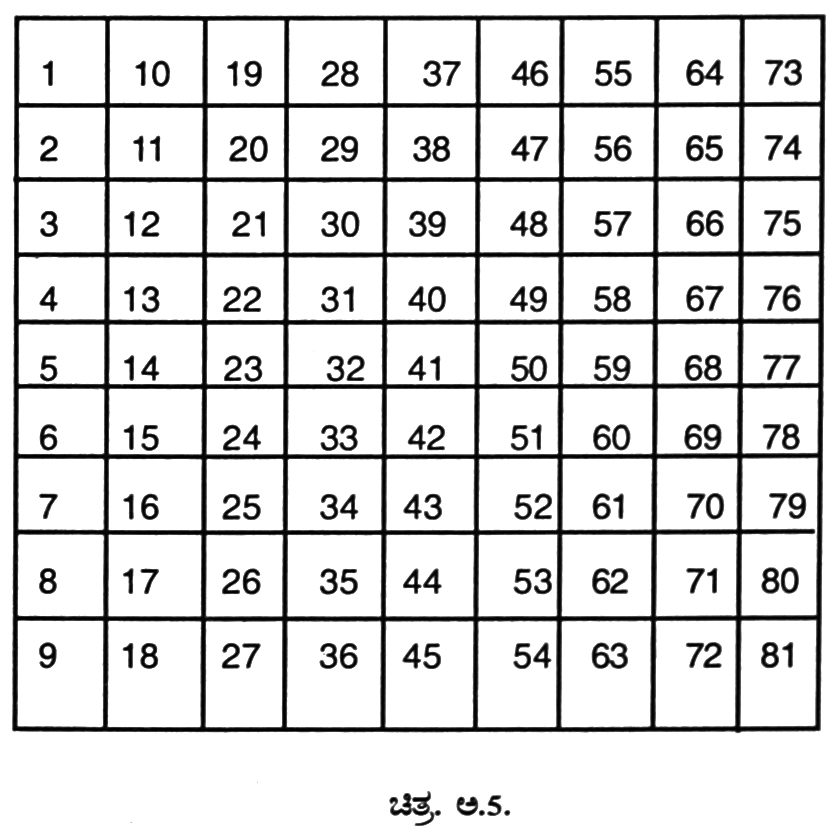
\includegraphics[scale=1.1]{src/figures/chap9/fig9-4.jpg}
\end{figure}
\begin{figure}[H]
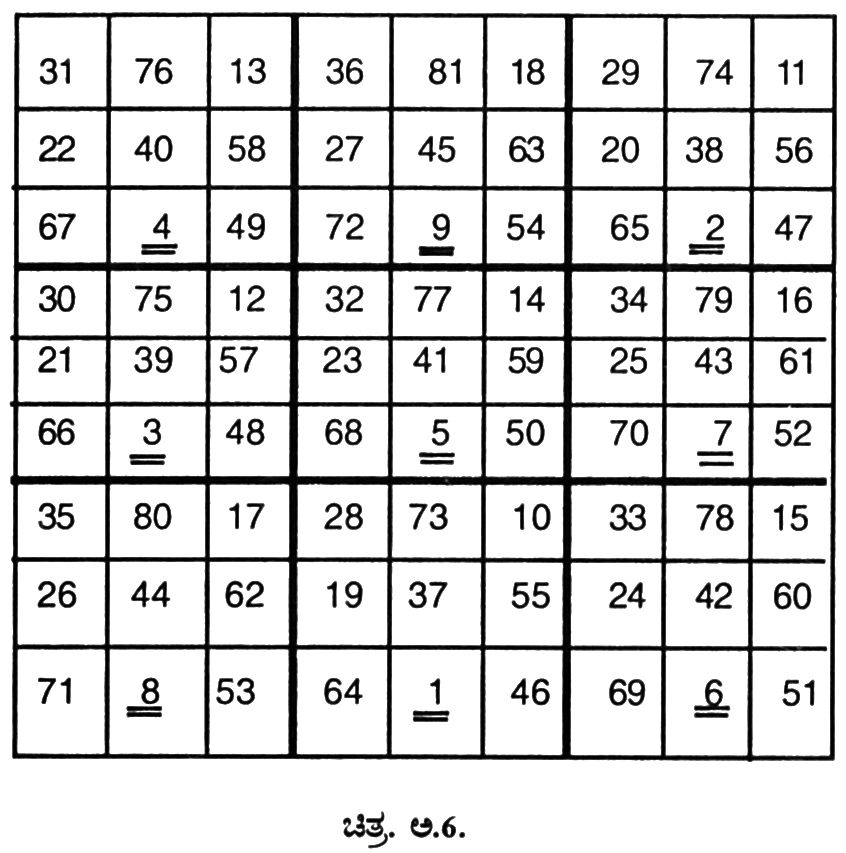
\includegraphics[scale=1.1]{src/figures/chap9/fig9-5.jpg}
\end{figure}

ಬೆಸ ಸಂಖ್ಯೆ ಕ್ರಮವರ್ಗದ ಮಾಯಾಚೌಕಗಳಲ್ಲಿ ಕೇಂದ್ರ ಸಂಖ್ಯೆಯು ಮಾಯಾಚೌಕದ ಅಕ್ಷವಾಗಿರುವುದು ಮಾತ್ರವಲ್ಲದೆ, ಒಟ್ಟಾರೆ ರಚನೆಗೆ ಆಧಾರವಾಗಿರುತ್ತದೆ. ಚೌಕದ ಸ್ಥಿರ ಮೊತ್ತ\-ವನ್ನು ಅಂದರೆ ಒಂದು ಸಾಲಿನ ಸಂಖ್ಯೆಗಳ ಮೊತ್ತವನ್ನು ನಿರ್ಧರಿಸುತ್ತದೆ. ಚೌಕದ ಎಲ್ಲ ಸಂಖ್ಯೆಗಳ ಒಟ್ಟನ್ನು ಪಡೆಯಲು ಸಹಾಯಕವಾಗುತ್ತದೆ. ಕೇಂದ್ರ ಸಂಖ್ಯೆಯ ಈ ಲಕ್ಷಣಗಳಿಂದಾಗಿ ಚೀನಾದ ಹ್ಯಾನ್ ಸಂತತಿಯವರು ಈ ಸಂಖ್ಯೆಯನ್ನು ಗೌರವಿಸುತ್ತಿದ್ದರು. ಹಾಗೂ ಈ ಸಂಖ್ಯೆಯನ್ನು ಅವರ ಮುಖ್ಯದೇವತೆಗಳಲ್ಲೊಂದಾದ ಟಾಯ್​ - ಇ ಮತ್ತು ಚೀನೀಯ ಚಕ್ರವರ್ತಿಯ ಸಂಗಡ ಜೊತೆಗೂಡಿಸುತ್ತಿದ್ದರು.

ಪ್ರಾಚೀನ ಚೀನೀಯರು 4 ಕ್ರಮವರ್ಗದ ಮಾಯಾಚೌಕವನ್ನು ರಚಿಸುತ್ತಿದ್ದ ವಿಧಾನವನ್ನು \textbf{ಯಾಂಗ್-ಹು-ಈ} ತಿಳಿಸುತ್ತಾನೆ. ಅದು ಹೀಗೆ ಇದೆ.

1 ರಿಂದ 16 ರವರೆಗಿನ ಕ್ರಮಾಗತ ಸಂಖ್ಯೆಗಳನ್ನು $4 \times 4$ ಚೌಕದಲ್ಲಿ ಕ್ರಮವಾಗಿ ತುಂಬಿಸುವುದು. (ಚಿತ್ರ. ಅ.7) ಅದರ ಕರ್ಣಗಳನ್ನು ತಿರುವು ಮುರುವು ಮಾಡಿ ಬರೆಯುವುದು ಮತ್ತು ಚೌಕವನ್ನು ಮೇಲಿನಿಂದ ಕೆಳಕ್ಕೆ ಎರಡು ಸಮ ಭಾಗಗಳಾಗಿ ಸೀಳುವುದು. (ಚಿತ್ರ.ಅ.8) ಈ ಭಾಗಗಳ ಸ್ಥಾನಗಳನ್ನು ಅದಲು ಬದಲು ಮಾಡಿ ಬರೆಯುವುದು. (ಚಿತ್ರ. ಅ.9) ಇದು ಮಾಯಾಚೌಕ.
\begin{figure}[H]
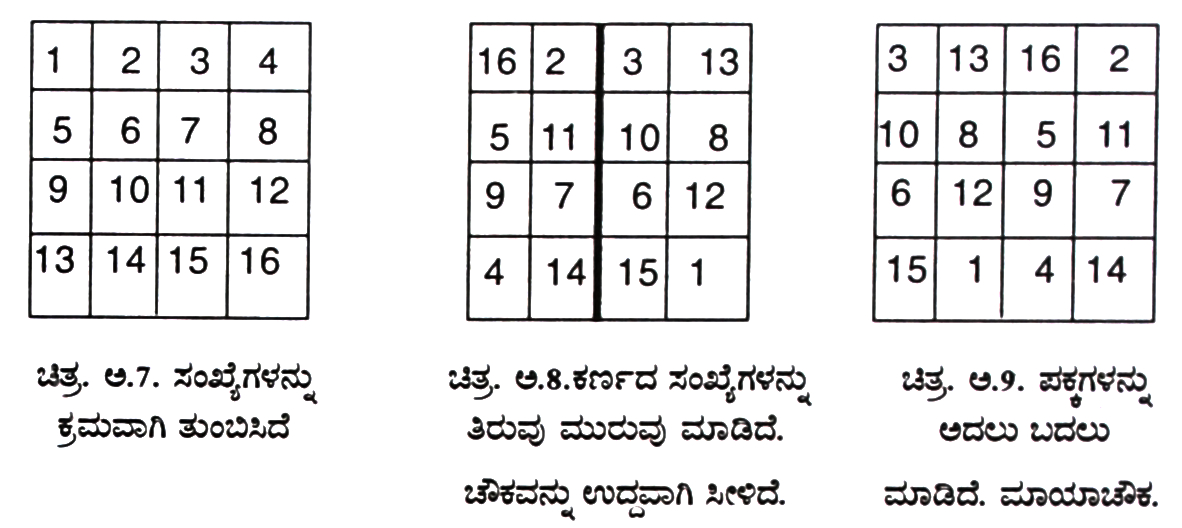
\includegraphics{src/figures/chap9/fig9-6.jpg}
\end{figure}

ಇದೇ ವಿಧಾನ ಅನುಸರಿಸಿ 8 ಕ್ರಮವರ್ಗದ ಮಾಯಾಚೌಕವನ್ನು ಚೀನೀಯರು ರಚಿಸಿದ ದಾಖಲೆ ಇದೆ.

ಲೋಷೂ ಚೌಕದ ಬಗೆಗೆ ಚೀನೀಯರಿಗೆ ಆರಾಧನಾ ಭಾವವಿದ್ದಿತು. 6 ಕ್ರಮವರ್ಗದ ಚೌಕ ರಚಿಸಲು ಯತ್ನಿಸಿದಾಗ ಲೋಷೂ ನಿಯಮವನ್ನು ಮುರಿಯಬೇಕಾಯಿತು. ಹಾಗಾಗಿ ಆ ಯತ್ನವನ್ನೇ ಕೈಬಿಡಲಾಯಿತು. ಆದರೂ 1593ರಲ್ಲಿ \textbf{ಚೆಂಗ್-ತಾ-ವೈ} ರಚಿಸಿದ 6 ಕ್ರಮವರ್ಗ ಚೌಕ ದೊರಕಿದೆ. \textbf{ಚೆಂಗ್-ತಾ-ವೈ} 1593ರಲ್ಲಿ ರಚಿಸಿದ್ದು.
\begin{figure}[H]
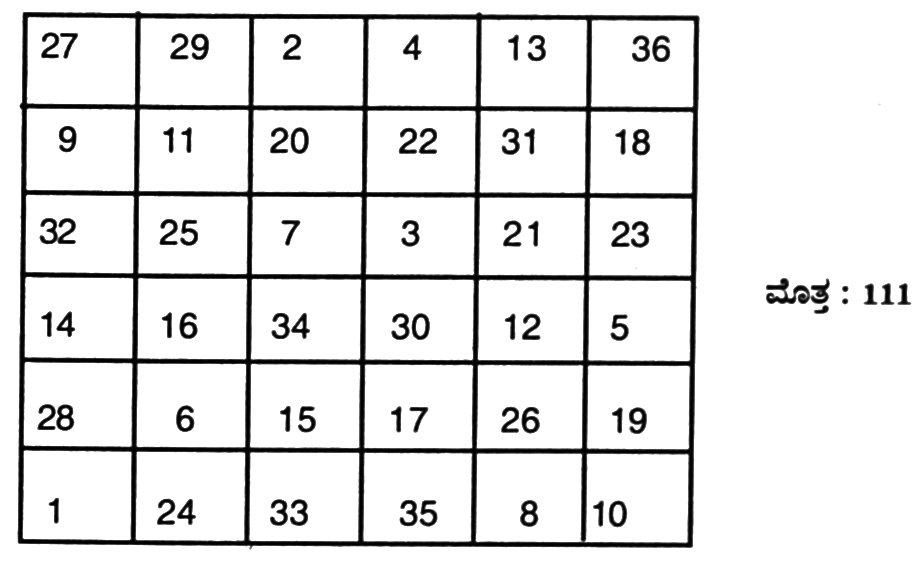
\includegraphics[scale=1.1]{src/figures/chap9/fig9-7.jpg}
\end{figure}

ಕ್ರಿ.ಶ. 9ನೇ ಶತಮಾನದ ಅಂತ್ಯದ ವೇಳೆಗೆ ಚೀನೀಯರಿಗೆ ಲೋಷೂ ಚೌಕದ ಬಗ್ಗೆ ಇದ್ದ ಗೌರವ ಕಡಿಮೆಯಾಯಿತು. ಅಲ್ಲಿಯವರೆಗೆ ಈ ಚೌಕಗಳಿಗೆ ಅತೀಂದ್ರಿಯ ಶಕ್ತಿ ಇರುವುದೆಂಬ ನಂಬಿಕೆಯಿಂದ ಅವುಗಳನ್ನು ನಿಗೂಢವಾಗಿ ಇರಿಸಲಾಗಿತ್ತು. ಅದರ ರಹಸ್ಯ ಬಯಲಾದಂತೆ ಮಾಯಾಚೌಕ ರಚನೆ ಎಲ್ಲರಿಗೂ ಎಟುಕುವಂತಾಗಿ, ಬಂದರು ನಗರಗಳಿಗೆ ಭೇಟಿ ನೀಡುತ್ತಿದ್ದ ಪರ್ಷಿಯಾ, ಅರೇಬಿಯಾ ಮತ್ತು ಭಾರತೀಯ ವರ್ತಕರಿಗೂ ಮಾಯಾಚೌಕಗಳ ಪರಿಚಯ ವಾಯಿತು. ಇವರಲ್ಲಿ ಯಾರು ಮೊದಲು ಕಲಿತರೆಂಬುದು ಮಾತ್ರ ತಿಳಿದುಬಂದಿಲ್ಲ.

\section*{ಮಧ್ಯಪ್ರಾಚ್ಯ :}

ಚೀನಾದಲ್ಲಿ ದೀರ್ಘಕಾಲದ ಪ್ರಯತ್ನದಿಂದ ಮಾಯಾಚೌಕಗಳ ಅಧ್ಯಯನ ಬೆಳೆದು ಬಂದಿದ್ದಿತು. ಸುಮಾರು ಕ್ರಿ.ಶ. 100 ವೇಳೆಗೆ ಕಾಗದದ ತಯಾರಿ ಆವಿಷ್ಕಾರವಾಯಿತು. ಇದರಿಂದಾಗಿ ಮಾಯಾಚೌಕಗಳ ಕುರಿತು ಅನೇಕ ಪ್ರಯೋಗಗಳು ನಡೆದು, ದಾಖಲಾದವು. ಪರ್ಷಿಯನ್ನರು ಮತ್ತು ಅರಬ್ಬರು ತಾವು ಸೆರೆಹಿಡಿದ ಚೀನೀ ಕುಶಲಕರ್ಮಿಗಳಿಂದ ಕಾಗದ ತಯಾರಿಯನ್ನು ಕಲಿತದ್ದೇ ಅಲ್ಲದೇ ಮಾಯಾಚೌಕಗಳ ರಚನೆಯನ್ನೂ ಕಲಿತರು. ಜೊತೆಗೆ ಹಿಂದೂಗಳಿಂದ ಸ್ಥಾನ ಬೆಲೆ ಸಂಖ್ಯೆ ಬರೆಯುವುದನ್ನು ತಿಳಿದುಕೊಂಡಿದ್ದ ಅವರಿಗೆ ಮಾಯಾಚೌಕಗಳ ಬಗ್ಗೆ ಕುತೂಹಲ \linebreak ಬಂದು, ಅದನ್ನು ಅಧ್ಯಯಿಸಿ ವಿಸ್ತಾರ ಮಾಡತೊಡಗಿದರು. ಕ್ರಿ.ಶ.900 ರ ಸುಮಾರಿಗೆ ಜಬೀರ್ ಇಬ್ನ್ ಹಯ್ಯಾನ್ ಎಂಬುವನು 3 ಕ್ರಮವರ್ಗದ ಮಾಯಾಚೌಕವನ್ನು ರಚಿಸಿದನೆಂದು ಹೇಳ\-ಲಾಗಿದೆ. ಮಾಯಾಚೌಕದ ರಚನೆಯ ಈ ವಿಧಾನವು ತೈನಾದ ಅಪೋಲೊನಿಯಸ್ನಿಂದ ದೊರಕಿ\-ತೆಂದೂ, ಇದನ್ನು ತಾಯಿತದಲ್ಲಿ ಕೆತ್ತಿಸಿ ಧರಿಸಿದರೆ ಸುಖಪ್ರಸವವಾಗುವುದೆಂದೂ ಅಜ್ಞಾತ ಲೇಖಕ\-ನೊಬ್ಬನ ಬರಹದಿಂದ ತಿಳಿದು ಬರುತ್ತದೆ. ಆದರೆ ವಾಸ್ತವವಾಗಿ ಮಾಯಾಚೌಕಗಳ \linebreak ವಿಚಾರ ಅರಬ್ಬರಿಗೆ ಲಭಿಸಿದುದು ಪೂರ್ವರಾಷ್ಟ್ರಗಳಾದ ಭಾರತ ಮತ್ತು ಚೀನಾಗಳಿಂದ.

ಮಾಯಾಚೌಕದ ಪ್ರವೇಶವು ಇಸ್ಲಾಮಿಕ್ ಸಂಸ್ಕೃತಿಯಲ್ಲಿ ತಾಯಿತದ ರೂಪದಲ್ಲಿ ಬೆಳೆದು ಬಂದು ಬಹಳ ಬೇಗ ಧಾರ್ಮಿಕ ಚೌಕಟ್ಟನ್ನು ಪ್ರವೇಶಿಸಿತು. ಕ್ರಿ.ಶ. 980ರಲ್ಲಿ ಬಾಸ್ರಾ ನಗರದಲ್ಲಿ ರಚಿತವಾದ ಅರಾಬಿಕ್ ವಿಶ್ವಕೋಶದಲ್ಲಿ ಕಂಡುಬರುವ ಮೂರರಿಂದ 9 ಕ್ರಮವರ್ಗದ ಮಾಯಾಚೌಕಗಳನ್ನು ಇಕ್ವಾನ್ ಅಸ್ ಸಫಾ ಎಂಬ ಇಸ್ಲಾಮೀ ಭ್ರಾತೃತ್ವ ಸಂಸ್ಥೆ ರಚಿಸಿತೆಂದು ನಂಬಲಾಗಿದೆ. ಹಲವಾರು ಹಸ್ತಪ್ರತಿಗಳು ದೊರೆತಿದ್ದು ಅವುಗಳಲ್ಲಿ ಭಿನ್ನತೆ ಕಂಡುಬರುತ್ತದೆ. ಆದರೆ ಒಟ್ಟಾರೆ ಲಕ್ಷಣಗಳು ಏಕ ರೀತಿಯಿದ್ದು ರಚನೆ ಹೇಳಿಸಿಕೊಳ್ಳುವಂಥದ್ದಲ್ಲ. 10ನೇ ಶತಮಾನದಲ್ಲಿನ ಇವು ಈ ಕ್ಷೇತ್ರದಲ್ಲಿ ಅನ್ಯರಿಂದ ಪಡೆದ ತಂತ್ರ ಬಳಸಿ ನಡೆಸಿದ ಪ್ರಯೋಗಗಳಾಗಿವೆ. ಚೀನೀಯರು ಲೋಷೂ ಬಗ್ಗೆ ಇರಿಸಿಕೊಂಡಿದ್ದ ರೀತಿ ಪವಿತ್ರ ಭಾವನೆಗಳನ್ನೇ ಇವರೂ ಸಹ ಹೊಂದಿದ್ದರೆಂದು ಹೇಳಬಹುದು.

ಸ್ವಾಭಾವಿಕ ಚೌಕದ ಅಂಕಿ/ಸಂಖ್ಯೆಗಳನ್ನು ಪ್ರತಿಲೋಮವಾಗಿಸಿ 3 ಮತ್ತು 4 ಕ್ರಮವರ್ಗದ ಸರಳ ಮಾಯಾಚೌಕಗಳ ರಚನೆಯ ನಂತರ 5 ಕ್ರಮ ವರ್ಗದ ಚೌಕ ರಚಿಸಲು ಯತ್ನಿಸಿರು\-ವುದು ಕಂಡುಬರುತ್ತದೆ. ಬಹುಶಃ 5ನೇ ವರ್ಗದ ಸ್ವಾಭಾವಿಕ ಚೌಕ ಬರೆದು, ಅದನ್ನು ವಜ್ರಾಕೃತಿ ಯಾಗು\-ವಂತೆ ಓರೆ ಮಾಡಿ, ಮಧ್ಯದ ಸಾಲುಗಳನ್ನು ತಿರುವು ಮುರುವು ಮಾಡಿ, ಉಳಿದ ಸಂಖ್ಯೆಗಳ ಜೊತೆಗಳನ್ನು ಪರಸ್ಪರ ಬದಲಾಯಿಸಿ, ವಜ್ರಾಕೃತಿಯನ್ನು ಚಪ್ಪಟೆ ಚೌಕವಾಗಿಸಿ ಮಾಯಾಚೌಕವನ್ನು ಪಡೆದಿರಬಹುದು. ಹಾಗೆಯೇ 8 ಮತ್ತು 9 ಕ್ರಮವರ್ಗದ ಚೌಕಗಳನ್ನು ರಚಿಸುವಲ್ಲಿ ಸಾಕಷ್ಟು ಶ್ರಮವಹಿಸಿರಬೇಕೆಂದು ಊಹಿಸಲಾಗಿದೆ. ಮೂರನೆ ಕ್ರಮವರ್ಗದ ಲೋಷೂ ಮಾದರಿ\-ಚೌಕ ರಚಿಸಿ, ಅದರ ಹೊರ ಸುತ್ತಲೂ ಸಂಖ್ಯೆಗಳನ್ನು ಹೊಂದಿಸಿ, 5 ಹಾಗೂ 7 ಕ್ರಮ\-ವರ್ಗದ ಆವರಣ ಮಾಯಾಚೌಕ ರಚನೆಯಲ್ಲಿ ಸಫಲರಾಗಿರುವುದು ತಿಳಿಯುತ್ತದೆ. ಪವಿತ್ರ ಭ್ರಾತೃ ಸಂಸ್ಥೆಯು (The Brethern of Purity) ಮಾಯಾಚೌಕ ರಚಿಸಲು ತಮ್ಮದೇ ಆದ ಎರಡು ವಿಧಾನಗಳನ್ನು ರೂಪಿಸಿಕೊಂಡರು. ಒಂದುವಿಧಾನದಲ್ಲಿ ಸಂಖ್ಯೆಗಳ ಬದಲು ಅಕ್ಷರಗಳನ್ನು ಬರೆದರು. ಇದನ್ನು ‘‘ಅಬ್ಜದ್’’ ವಿಧಾನ ಎನ್ನಲಾಗಿದೆ. ಇನ್ನೊಂದು ವಿಧಾನದಲ್ಲಿ ಸಂಖ್ಯೆ\-ಗಳನ್ನು ಚದುರಂಗದ ಕುದುರೆ ನಡಿಗೆಯ ಮಾದರಿಯಲ್ಲಿ ತುಂಬಿಸಲಾಗಿದೆ. ಚೀನೀ \break ಮಾದರಿಯ ಜಡ ಪದ್ದತಿಗಿಂತ ಇದು ಸ್ಥಾಯೀ ಆಗಿದ್ದು ಮುಂದೆ ಹೊಸ ಹೊಸ ರೀತಿಯ ಚೌಕಗಳ ರಚನೆಗೆ ನಾಂದಿಯಾಯಿತು.

ಅತಿ ಶೀಘ್ರದಲ್ಲಿ ಮಧ್ಯಪ್ರಾಚ್ಯದ ಗಣಿತಜ್ಞರು ಬೆಸಸಂಖ್ಯೆ ಕ್ರಮವರ್ಗದ ಮಾಯಾಚೌಕ ಗಳನ್ನು ಅನುಕ್ರಮ ಸಂಖ್ಯೆಗಳಿಂದ ರಚಿಸುವ ವಿಧಾನ ಕಂಡುಕೊಂಡರು. ಇವರು 1ನ್ನು ಚೌಕದ\-ಕೇಂದ್ರ ಮನೆಯ ಕೆಳಗಿನ ಮನೆಯಲ್ಲಿ ಬರೆದು, ಮುಂದಿನ ಕ್ರಮಾಗತ ಸಂಖ್ಯೆಗಳನ್ನು ಓರೆಯಾಗಿ ಬಲ ಕೆಳಗಡೆಗೆ ಇರುವ ಮನೆಗಳಲ್ಲಿ ತುಂಬಿಸಿದರು. ತಳಗಡೆ ಕೊನೆ ಮನೆ ತಲುಪಿದ ನಂತರ ಮುಂದಿನ ಕಂಭಸಾಲಿನ ಮೇಲ್ತುದಿಯ ಮನೆಯನ್ನು ತುಂಬಿಸಿದರು. ಬಲಗಡೆ ಮನೆ ಇಲ್ಲದಾಗ ಅದೇ ಅಡ್ಡಸಾಲಿನ ಮೊದಲ ಮನೆ ತುಂಬಿಸಿದರು. ಮುಂದಿನ ಮನೆ ಆದಾಗಲೇ \linebreak ತುಂಬಲ್ಪಟ್ಟಿದ್ದರೆ ಅದೇ ಸಾಲಿನ ಕೆಳತುದಿಯ ಮನೆಯನ್ನು ತುಂಬಿಸಿದರು. ಇದೇ ಕ್ರಮದಲ್ಲಿ ಎಲ್ಲ ಮನೆಗಳನ್ನು ತುಂಬಿಸಿ ಮಾಯಾಚೌಕವನ್ನು ಪಡೆದರು. (ಚಿತ್ರ.ಅ.10)
\begin{figure}[H]
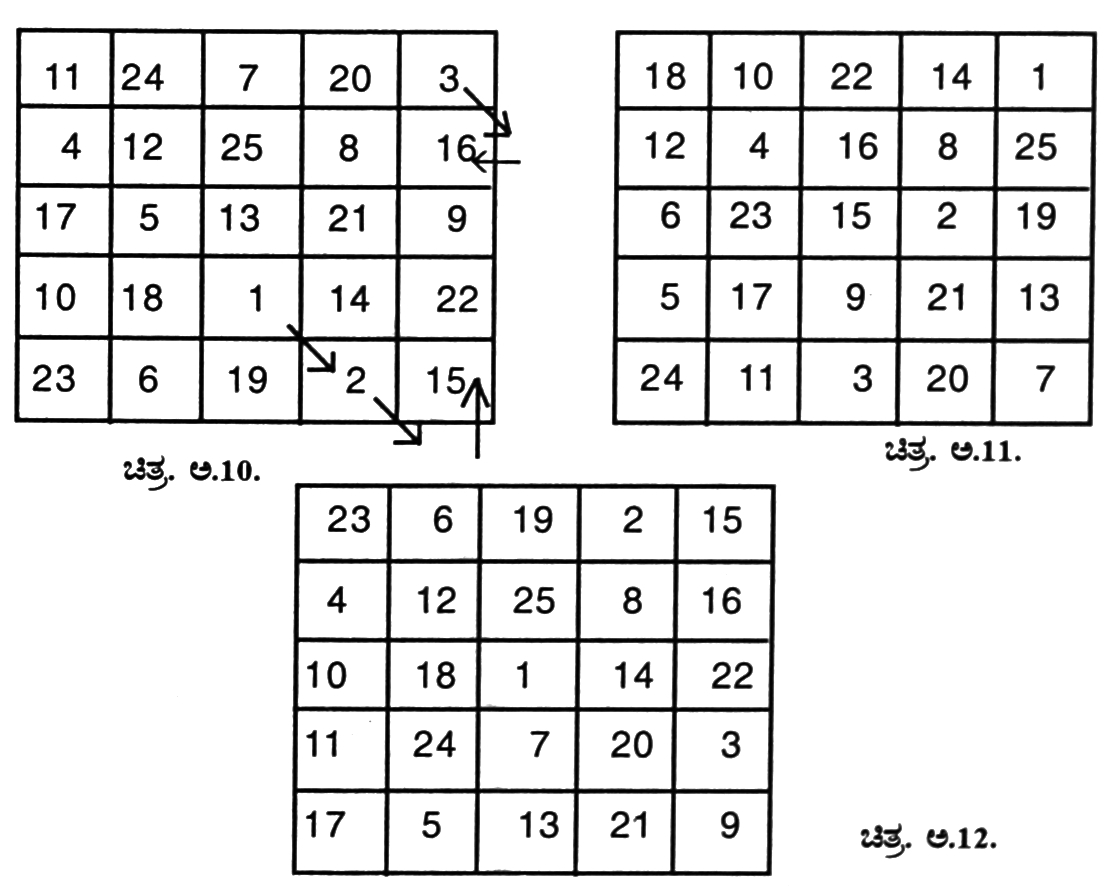
\includegraphics{src/figures/chap9/fig9-8.jpg}
\end{figure}

ಭಾರತೀಯರಿಂದ ಕಲಿತಿದ್ದ ಚದುರಂಗ ಆಟದಲ್ಲಿನ ಕುದುರೆ ನಡೆಯನ್ನು ಮಾಯಾ\-ಚೌಕದಲ್ಲಿ ಬಳಸಿದರು. (ಯಾವುದೇ ಪಕ್ಕಕ್ಕೆ 2ಮನೆ, ಅಲ್ಲಿಂದ 1ಮನೆ), ಕೆಲವೊಮ್ಮೆ ಇಂತಹ ಮಾಯಾ\-ಚೌಕಗಳ, ರಚನೆಯಲ್ಲಿ, ಹಲವು ಮಾರ್ಪಾಡುಗಳನ್ನು ಮಾಡಿದರು. (ಚಿತ್ರ.ಅ.11) ಕುದುರೆ ನಡೆಯ ಮಾಯಾಚೌಕಗಳಲ್ಲಿ ಕೇಂದ್ರ ಮನೆಯಲ್ಲಿ 1ನ್ನು ತುಂಬಿಸಿ ರಚಿಸಿದವುಗಳನ್ನು ಪವಿತ್ರವೆಂದು ಭಾವಿಸಲಾಗಿದ್ದಿತು. 1 ಎನ್ನುವುದು ಸೃಷ್ಟಿಕರ್ತ ಅಲ್ಲಾಹುರವರನ್ನು ಪ್ರತಿನಿಧಿಸಿದೆಯೆಂದು ನಂಬಲಾಗಿದ್ದಿತು.

ಸಾಮಾನ್ಯವಾಗಿ ಚದುರಂಗದ ಕುದುರೆ ನಡಿಗೆಯ ಮಾಯಾಚೌಕಗಳು ಸರ್ವತೋಮುಖ (Pandiagonal) ಮಾಯಾಚೌಕಗಳು. ಇವುಗಳಲ್ಲಿ ಉಪಕರ್ಣಗಳ ಸಂಖ್ಯೆಗಳ ಮೊತ್ತವೂ ಮಾಯಾಮೊತ್ತಕ್ಕೆ ಸಮ. ಉದಾಹರಣೆಗೆ : ಅ. 11 ಚಿತ್ರದಲ್ಲಿ 6+4+22+20+13=65; ಇದೇ ರೀತಿ 24+10+16+2+13=65 ಇಸ್ಲಾಮಿಕ್ ಗಣಿತಜ್ಞರ ಕೇಂದ್ರ ಮನೆಯಲ್ಲಿ 1 ಇರುವ ಮಾಯಾಚೌಕಗಳು ವಿವಿಧ ರೀತಿಗಳಲ್ಲಿ ರಚಿಸಲ್ಪಟ್ಟು ರಹಸ್ಯಮಯವಾಗಿ ಕಾಣುತ್ತವೆ.

ಅರಬ್ಬರು 4 ಕ್ರಮವರ್ಗದ ಮಾಯಾಚೌಕವನ್ನು ಕೆಲವು ಬದಲಾವಣೆಗೆ ಒಳಪಡಿಸಿ ಸರ್ವತೋಮುಖ ಚೌಕಗಳನ್ನು ರಚಿಸಿದ್ದಾರೆ.

ಈ ಚೌಕದಲ್ಲಿ :13+11+4+6 = 34

14+12+3+5 = 34

3+2+14+15=34

13+16+4+1 = 34

11+7+6+10=34
\begin{figure}[H]
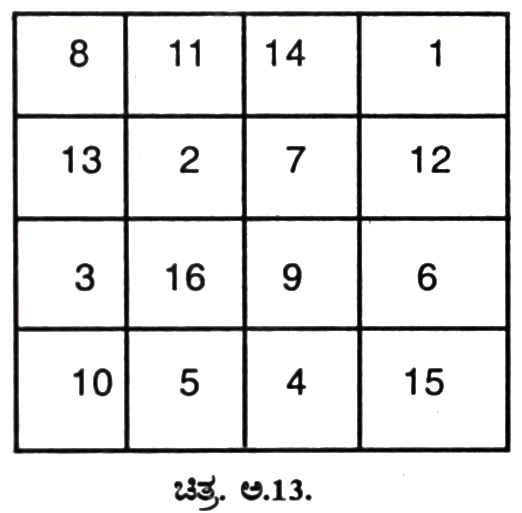
\includegraphics{src/figures/chap9/fig9-9.jpg}
\end{figure}

ಪರ್ಷಿಯನ್ ಮತ್ತು ಅರಾಬಿಕ್ ಗಣಿತಜ್ಞರು 4 ಕ್ರಮವರ್ಗದ ಮಾಯಾಚೌಕಗಳ ವಿಶಿಷ್ಟತೆ ಮತ್ತು ವೈಚಿತ್ರ್ಯವನ್ನು ಮನಗಂಡು, ಅವುಗಳಲ್ಲಿ ಯಾವುದೋ ಶಕ್ತಿ ಇರಬಹುದೆಂದು ಭಾವಿಸಿದರು. ಇವು ಒಳಿತು ಅಥವಾ ಕೆಡುಕನ್ನು ಮಾಡಬಹುದೆಂದು ನಂಬಿದರು. ಆ ಕಾರಣದಿಂದಾಗಿ ಹೋರಾಟದಲ್ಲಿ ಬಳಸುವ ಕತ್ತಿಯ ಅಲಗಿನ ಮೇಲೆ ಚೌಕವನ್ನು ಕೊರೆಯಿಸಿ, ಖಡ್ಗದ ಛೇದಿಸುವ ಶಕ್ತಿ ವೃದ್ಧಿಸಲು ಯತ್ನಿಸಿದರು. ಹಲವರು ಲೋಹದ ಬೋಗುಣಿಗಳ ಒಳಗೆ ಕೆತ್ತಿಸಿ, ಅಂತಹ ಬೋಗುಣಿಯ ಒಳಗೆ ಹಾಕಿದ ವಸ್ತುಗಳು ಶುದ್ಧವಾಗುತ್ತವೆಂದು ಪರಿಗಣಿಸಿದರು.

8 ಮತ್ತು 12 ಕ್ರಮವರ್ಗಗಳ ಮಾಯಾಚೌಕಗಳನ್ನು ರಚಿಸಲು ಅನುಕ್ರಮ ಸಂಖ್ಯೆಗಳನ್ನು ಬಳಸಿದರು. ಇದರಲ್ಲಿ 4 ಕ್ರಮವರ್ಗದ ಚೌಕ ರಚನೆಯ ಅನುಭವವನ್ನು ಉಪಯೋಗಿಸಿದರು. ಇಷ್ಟೇ ಅಲ್ಲದೆ 3 ಮತ್ತು 5 ಕ್ರಮವರ್ಗದ ಚೌಕಗಳನ್ನು 4 ಕ್ರಮವರ್ಗದ ಚೌಕಗಳೊಡನೆ ಜೋಡಿಸಿ, ದೊಡ್ಡ ಸಂಯುಕ್ತ ಮಾಯಾಚೌಕಗಳನ್ನು ರಚಿಸಿದರು. ಉದಾಹರಣೆಗೆ 20 ಕ್ರಮ\-ವರ್ಗದ ಮಾಯಾಚೌಕ ರಚಿಸಲು 1 ರಿಂದ 400 ವರೆಗಿನ ಸಂಖ್ಯೆಗಳನ್ನು ಬಳಸಿ 5 ಕ್ರಮವರ್ಗದ 16 ಮಾಯಾಚೌಕಗಳನ್ನು ರಚಿಸಿದರು. ಅವುಗಳನ್ನು 4 ಕ್ರಮವರ್ಗದ ಸರ್ವತೋಮುಖ \break ಮಾಯಾಚೌಕದ ಮಾದರಿಯಲ್ಲಿ ಜೋಡಿಸಿ 20 ಕ್ರಮವರ್ಗದ ಚೌಕ ಪಡೆದರು.

ಚೀಣೀಯರ ಆವರಣ ಮಾಯಾಚೌಕಗಳ ರಚನೆಯನ್ನು ಉತ್ತಮಗೊಳಿಸಿದುದು ಇಸ್ಲಾಮಿಕ್ ಗಣಿತಜ್ಞರ ವಿಶೇಷ ಕೊಡುಗೆ. ಈ ವಿಧಾನವನ್ನು ಕ್ರಿ.ಶ. 1225 ರಲ್ಲಿ \textbf{ಮುಹ್ಯಿಲ್ ದೀನ್ ಅಬು ಇ ಅಬ್ಬಾಸ್ಲ್ಬೂನಿ } ಎಂಬ ಉತ್ತರ ಆಫ್ರಿಕಾದ ವಿದ್ಯಾರ್ಥಿಯು ವಿವರಿಸಿದ್ದಾನೆ. \hbox{ತಾನೇ ಇದರ ಕರ್ತೃ} ಎಂದು ಹೇಳಿಕೊಂಡಿಲ್ಲ. ಬೆಸ ಸಂಖ್ಯೆ ಕ್ರಮವರ್ಗದ ಆವರಣ ಮಾಯಾಚೌಕ ರಚಿಸಲು 3 ಕ್ರಮವರ್ಗದ ಮಾಯಾಚೌಕವನ್ನು ಆಧಾರವಾಗಿಸಿಕೊಂಡನು. ಅದರಲ್ಲಿ ಶ್ರೇಢಿಯ ಮೊದಲ ಮೂರು, ಮಧ್ಯದ ಮೂರು ಹಾಗೂ ಕಡೆಯ ಮೂರುಸಂಖ್ಯೆಗಳನ್ನು ಬಳಸಿದನು. ಉಳಿದ ಸಂಖ್ಯೆಗಳನ್ನು ಚೌಕದ ಹೊರಸುತ್ತಿನ ಮನೆಗಳಲ್ಲಿ ಎದುರು ಬದುರು ಮನೆಗಳ ಸಂಖ್ಯೆಗಳ ಮೊತ್ತ ಒಂದೇ ಸಮವಾಗಿರುವಂತೆ ಅಂಕು ಡೊಂಕು (Zig-Zag) ರೀತಿಯಲ್ಲಿ \break ತುಂಬಿಸಿದ. ಇದೇ ರೀತಿ ಸಮಸಂಖ್ಯೆ ಕ್ರಮವರ್ಗದ ಚೌಕ ರಚಿಸಲು 4 ಕ್ರಮವರ್ಗದ ಚೌಕ\-ವನ್ನು ಆಧಾರವಾಗಿಸಿಕೊಂಡನು. ಅದರ ಹೊರಸುತ್ತಿನ ಮನೆಗಳಲ್ಲಿ ಉಳಿದ ಸಂಖ್ಯೆಗಳನ್ನು ಅಂಕು\-ಡೊಂಕು (Zig-Zag) ರೀತಿಯಲ್ಲಿ ಎದುರು ಬದುರು ಮನೆಗಳ ಸಂಖ್ಯೆಗಳ ಮೊತ್ತ ಸಮನಾಗಿರುವಂತೆ ತುಂಬಿಸಿದ. ಇವುಗಳ ರಚನೆಯಲ್ಲಿ ಅಲ್ ಬೂನಿಯ ಚತುರತೆ ಚೆನ್ನಾಗಿ ಮೂಡಿಬಂದಿದೆ. ಇಂತಹ ಚೌಕಗಳು ಜೀವಿಯ ಹುಟ್ಟು ಮತ್ತು ಆತ್ಮದ ಪಥದ ಸೂಚಕ ಎಂದು ಕಲ್ಪಿಸಲಾಗಿತ್ತು.
\begin{figure}[H]
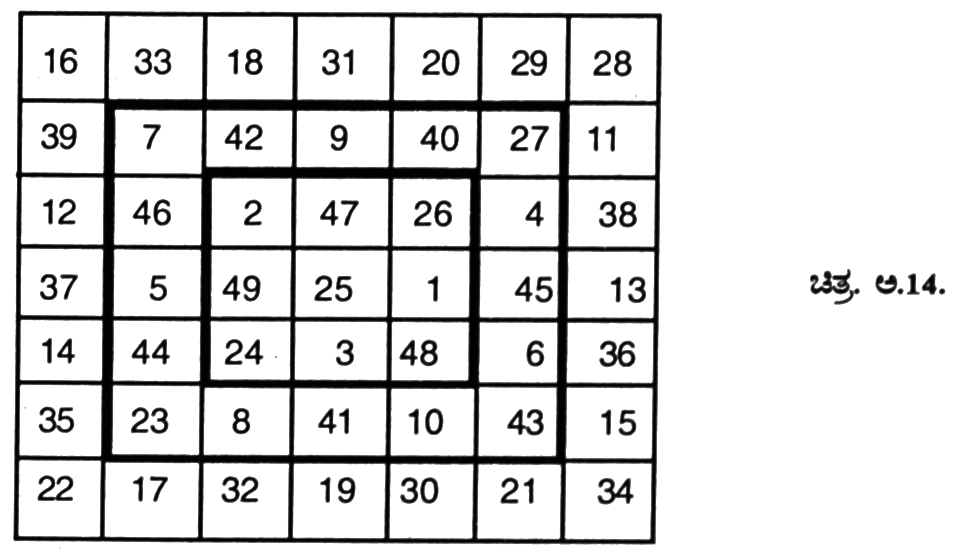
\includegraphics[scale=.85]{src/figures/chap9/fig9-10.jpg}
\end{figure}
\begin{figure}[H]
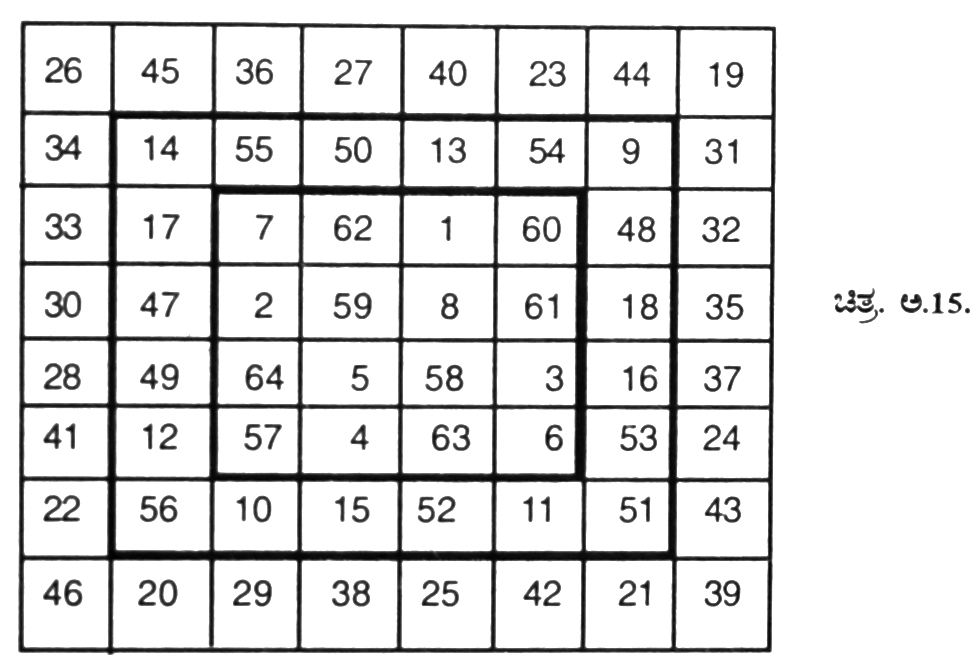
\includegraphics[scale=.85]{src/figures/chap9/fig9-11.jpg}
\end{figure}

ಅಲ್ಬೂನಿ ಮತ್ತು ಆ ಕಾಲದ ಗಣಿತಜ್ಞರು ಸಂಖ್ಯೆಗಳ ಜೋಡಣೆಯನ್ನು ಬದಲಾಯಿಸಿ, ಬೇರೆ ಬೇರೆ ಚೌಕಗಳನ್ನು ರಚಿಸುವಲ್ಲಿ ಯಶಸ್ವಿಯಾದರು. $30 \times 30$ ಚೌಕವನ್ನು ಅವರು ರಚಿಸಿದ ಬಗೆಗೆ ದಾಖಲೆ ಇದೆ. ಸಮ ಮತ್ತು ಬೆಸ ಸಂಖ್ಯೆ ಕ್ರಮವರ್ಗದ ಆವರಣ ಚೌಕಗಳನ್ನು ರಚಿಸುವ ಇವರ ವಿಧಾನ ಕ್ರಿ.ಶ.1540ರ ಸುಮಾರಿಗೆ ಯುರೋಪನ್ನು  ಪ್ರವೇಶಿಸಿ, ಇಪ್ಪತ್ತನೆಯ ಶತಮಾನದ ವರೆವಿಗೂ ಯಾವ ಬದಲಾವಣೆಯೂ ಇಲ್ಲದೇ ಬಳಕೆಯಾಗುತ್ತಿದ್ದುದು ಮೆಚ್ಚುಗೆಯ ವಿಷಯವೇ ಸರಿ.

\section*{ಭಾರತ :}

ಅನೇಕ ಗಣಿತ ಇತಿಹಾಸಕಾರರ ದೃಷ್ಟಿಯಲ್ಲಿ ಮಾಯಾಚೌಕಗಳು ಹಿಂದೂಗಳಿಗೆ ಪುರಾತನ ಕಾಲದಿಂದಲೇ ಪರಿಚಿತವಾಗಿತ್ತೆಂಬುದು ವೇದ್ಯವಾಗುತ್ತದೆ. ಆದರೆ ಲಭ್ಯ ಅತಿ ಪುರಾತನ ಮಾಯಾ\-ಚೌಕವೆಂದರೆ, ಕ್ರಿ.ಶ. 12 ಮತ್ತು 13ನೆಯ ಶತಮಾನಗಳದ್ದು. ಮುಸ್ಲಿಮರ ಆಕ್ರಮಣದ \hbox{ನಂತರದ} ಅವಧಿಯದು. ಈ ಕಾಲದ ಎರಡು ವಿಭಿನ್ನ ಮಾಯಾಚೌಕಗಳು ದೊರೆತಿವೆ. ಅವು ನಾಲ್ಕನೆಯ ಕ್ರಮವರ್ಗದವು. ಅವುಗಳಲ್ಲೊಂದು ಇಸ್ಲಾಮಿಕ್ ಚೌಕಗಳನ್ನು ಹೋಲುತ್ತದೆ; ಮತ್ತೊಂದು ಆ ಚೌಕದಿಂದ ವ್ಯುತ್ಪನ್ನ ಮಾಡಿದುದಾಗಿದೆ.

ಹಿಂದೂ ಗಣಿತಜ್ಞರು 4 ಕ್ರಮವರ್ಗದ ಮಾಯಾಚೌಕಗಳನ್ನು ಅನೇಕ ರೀತಿಯ ಪ್ರಯೋಗ\-ಗಳಿಗೆ ಒಳಪಡಿಸಿದರು. ಅವು ಬಹಳ ಪರಿಣಾಮಕಾರಿಯೆಂದು ಭಾವಿಸಿ ಅವುಗಳನ್ನು ರಕ್ಷಾಯಂತ್ರ ಮತ್ತು ತಾಯಿತಗಳಲ್ಲಿ ಕೆತ್ತಿಸಿ, ಧರಿಸತೊಡಗಿದರು. ಕ್ರಿ.ಶ. 19ನೆಯ ಶತಮಾನದಲ್ಲಿ ಎ.ಎಚ್. ಫ್ರಾಸ್ಟ್ ಎಂಬ ಕ್ರಿಶ್ಚಿಯನ್ ಮತಪ್ರಚಾರಕನು ನಾಸಿಕ ಪಟ್ಟಣದಲ್ಲಿ 4 ಕ್ರಮವರ್ಗದ ಒಂದು ಮಾಯಾಚೌಕವನ್ನು ಪತ್ತೆಮಾಡಿದನು. ಇದು ಒಂದು ಸರ್ವತೋಮುಖ ಮಾಯಾಚೌಕ. ಇದನ್ನು \textbf{‘ನಾಸಿಕ್ ಮಾಯಾಚೌಕ’} ಎಂದು ಕರೆಯಲಾಯಿತು. (ವಿವರಗಳು ಪುಟ 46 ರಲ್ಲಿವೆ)

ಭಾರತದಲ್ಲಿ ಮಾಯಾಚೌಕಗಳ ಅಧ್ಯಯನ ಬಹಳ ಪ್ರಾಚೀನವಾದದ್ದೆಂಬ ವಾದವಿದ್ದರೂ ಅದನ್ನು ಪುಷ್ಟೀಕರಿಸುವ ಲಿಖಿತ ಆಧಾರಗಳು ಲಭ್ಯವಾಗಿಲ್ಲ. ಆದರೆ ಕ್ರಿ.ಶ. 1356ರ ವೇಳೆಗೆ \hbox{ನಾರಾಯಣ} ಪಂಡಿತನಿಂದ ರಚಿತವಾದ ‘‘ಗಣಿತ ಕೌಮುದಿ’’ ಎಂಬ ಗ್ರಂಥವನ್ನು ಪರಿಶೀಲಿಸಿದಾಗ ಮಾಯಾಚೌಕಗಳ ಬಗೆಗೆ ಅಧ್ಯಯನವು ಉನ್ನತ ಮಟ್ಟದ್ದಾಗಿತ್ತೆಂಬುದು ತಿಳಿದು ಬರುತ್ತದೆ. ಇದರಲ್ಲಿನ ಮಾಯಾಚೌಕಗಳ ರಚನಾವಿಧಾನವು ಭಗವಾನ್ ಶಿವ (ದೇವರು) ನಿಂದ ಪೌರಾಣಿಕ ರಾಜನೊಬ್ಬನಿಗೆ ಬೋಧಿಸಲ್ಪಟ್ಟಿತೆಂಬ ದಂತಕಥೆಯೂ ಪ್ರಚುರವಾಗಿದ್ದಿತು. ಈ ಗ್ರಂಥದಲ್ಲಿ 4 ಮತ್ತು 8 ಕ್ರಮವರ್ಗಗಳ ಅನೇಕ ವಿಧವಾದ ಮಾಯಾಚೌಕಗಳ ವಿವರಗಳಿವೆ. \hbox{ಅವುಗಳ ರಚನೆ} ಪೂರ್ಣವಾಗಿ ಭಾರತೀಯವೇ ಎಂಬುದು ಗಮನಾರ್ಹ ಅಂಶ.
\eject

ಮಾಯಾಚೌಕ ರಚನೆಗೆ ನಾರಾಯಣ ಪಂಡಿತನಿಂದ ವಿವರಿಸಲ್ಪಟ್ಟಿರುವ ಒಂದು ತಂತ್ರ \hbox{ಹೀಗಿದೆ.} ಎರಡು ಸಹಾಯಕ ಚೌಕಗಳನ್ನು ರಚಿಸಿ, ಅವುಗಳನ್ನು ಒಂದುಗೂಡಿಸಿ ಮಾಯಾಚೌಕ ವನ್ನು ಪಡೆಯುವುದು. ಉದಾಹರಣೆಗೆ 5 ಕ್ರಮವರ್ಗದ ಮಾಯಾಚೌಕ ರಚಿಸಬೇಕೆಂದಿಟ್ಟು ಕೊಳ್ಳೋಣ. ಮೊದಲು $5 \times 5$ಚೌಕದ ಮಧ್ಯದ ಕಂಭಸಾಲಿನಲ್ಲಿ 1 ರಿಂದ 5 ರ ವರೆಗಿನ ಸಂಖ್ಯೆ\-ಗಳನ್ನು ಯಾವುದೇ ಕ್ರಮದಲ್ಲಿ ತುಂಬಿಸುವುದು. ಸಂಖ್ಯೆಗಳನ್ನು ಎಡಕೆಳಗೆ ಮತ್ತು ಬಲ ಮೇಲಕ್ಕೆ ಓರೆಯಾಗಿ ತುಂಬಿಸುವುದು. (ಚಿತ್ರ. ಅ.16) ಮತ್ತೆ ಎರಡನೆ $5 \times 5$ ಚೌಕದ ಮಧ್ಯದ ಕಂಭ ಸಾಲಿನಲ್ಲಿ 0,5,10,15,20 ಸಂಖ್ಯೆಗಳನ್ನು ಕ್ರಮವಾಗಿ ಮೇಲಿನಿಂದ ಕೆಳಕ್ಕೆ ತುಂಬಿಸುವುದು. ಈ ಚೌಕದ ಮನೆಗಳನ್ನು ಓರೆಯಾಗಿ ಎಡ ಕೆಳಕ್ಕೂ ಹಾಗೂ ಬಲ ಮೇಲಕ್ಕೂ ತುಂಬಿಸುವುದು. \linebreak (ಚಿತ್ರ. ಅ. 17) ಮೂರನೆಯ $5 \times 5$ ಚೌಕದಲ್ಲಿ ಮೊದಲೆರಡು ಚೌಕಗಳ ಸಂಖ್ಯೆಗಳನ್ನು ಕೆಳ ಕಾಣಿಸಿರುವಂತೆ ತುಂಬಿಸುವುದು.

\smallskip
\noindent ಅ.16 ಚೌಕದ 1ನೆ ಕಂಭಸಾಲು + ಅ.17. 5ನೆ ಕಂಭಸಾಲು ಅ.18.ಚೌಕದ 1 ಕಂಭಸಾಲು

\smallskip
\noindent ಅ.16 ಚೌಕದ 2ನೆ ಕಂಭಸಾಲು+ಅ.17. 4ನೆ ಕಂಭಸಾಲು ಅ.18. ಚೌಕದ 2 ಕಂಭಸಾಲು

\smallskip
\noindent ಅ.16 ಚೌಕದ 3ನೆ ಕಂಭಸಾಲು + ಅ.17. 3ನೆ ಕಂಭಸಾಲು ಅ.18.ಚೌಕದ 3 ಕಂಭಸಾಲು

\smallskip
\noindent ಅ.16 ಚೌಕದ 4ನೆ ಕಂಭಸಾಲು + ಅ.17. 2ನೆ ಕಂಭಸಾಲು ಅ.18.ಚೌಕದ 4 ಕಂಭಸಾಲು

\smallskip
\noindent ಅ.16 ಚೌಕದ 5ನೆ ಕಂಭಸಾಲು + ಅ.17. 1ನೆ ಕಂಭಸಾಲು ಅ.18. ಚೌಕದ 5 ಕಂಭಸಾಲು

\smallskip
\noindent ಅ.18 ಚಿತ್ರದ ಚೌಕವು 5 ಕ್ರಮವರ್ಗದ ಮಾಯಾಚೌಕ
\begin{figure}[H]
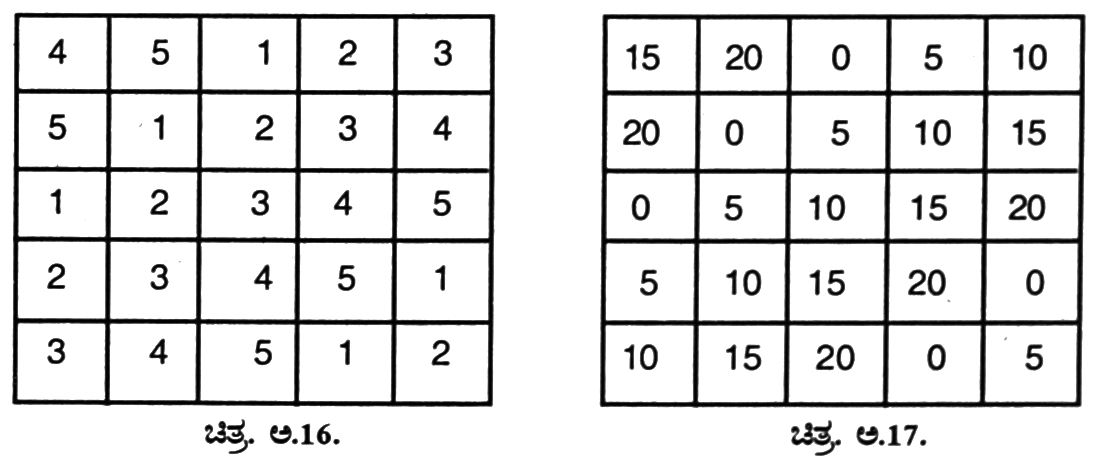
\includegraphics[scale=1.15]{src/figures/chap9/fig9-12.jpg}
\end{figure}
\begin{figure}[H]
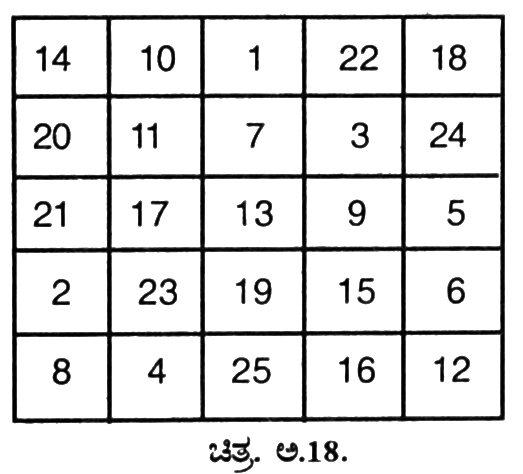
\includegraphics{src/figures/chap9/fig9-13.jpg}
\end{figure}

ಚಿತ್ರ ಅ. 18 ರಲ್ಲಿನ ಮಾಯಾಚೌಕದ ಮೊತ್ತ 65

ಈ ವಿಧಾನದಿಂದ ಯಾವುದೇ ಬೆಸಸಂಖ್ಯೆ ಕ್ರಮವರ್ಗದ ಮಾಯಾಚೌಕವನ್ನು ರಚಿಸ\-ಬಹುದು. ಈ ವಿಧಾನ ಅಂದರೆ ಚೌಕಗಳನ್ನು ರಚಿಸಿ ಒಟ್ಟು ಮಾಡುವುದರಿಂದ 4 ಮತ್ತು 8 ಕ್ರಮ\-ವರ್ಗಗಳ ಮಾಯಾಚೌಕಗಳನ್ನು ನಾರಾಯಣ ಪಂಡಿತನು ರಚಿಸಿದ್ದಾನೆ. ಅವುಗಳಲ್ಲಿ ಸಂಖ್ಯೆ\-ಗಳನ್ನು ತುಂಬಿಸುವ ಕ್ರಮ ಬೇರೆಯದೇ ಆಗಿದೆ. $2 \times 2$ರ ಸಹಾಯಕ ಚೌಕಗಳನ್ನು ರಚಿಸಿ, ಅವುಗಳನ್ನು ವಿಶಿಷ್ಟ ರೀತಿಯಾಗಿ ಜೋಡಿಸಿ ಮಾಯಾಚೌಕಗಳನ್ನು ಪಡೆಯಲಾಗಿದೆ. ಇವುಗಳಲ್ಲಿ ಸಂಖ್ಯೆಗಳ ಸಾಲುಗಳು ಪರಸ್ಪರ ವಿರುದ್ಧ ದಿಕ್ಕಿನಲ್ಲಿ ಕ್ರಮಿಸಿ, ಇಡೀ ನಮೂನೆಯು ಸೃಷ್ಟಿಯ ಜಾಲವನ್ನು ಹೋಲುತ್ತದೆಂಬ ನಂಬಿಕೆಯಿಂದಾಗಿ ಈ ಚೌಕಗಳನ್ನು ಪವಿತ್ರ ಎಂದು ಭಾವಿಸ\-ಲಾಗಿದ್ದಿತು.

ನಾರಾಯಣ ಪಂಡಿತನ ನಂತರ 3 ಶತಮಾನಗಳಿಗಿಂತ ಹೆಚ್ಚು ಕಾಲವಾದ ಮೇಲೆ \linebreak ಫಿಲಿಪ್ ಡಿ ಲಾ ಹೈರ್ (1640-1718) ಎಂಬ ಫ್ರೆಂಚ್ ಗಣಿತಜ್ಞನು ಇದೇ ವಿಧಾನವನ್ನು ಅನುಸರಿಸಿ ಮಾಯಾಚೌಕಗಳನ್ನು ರಚಿಸಿದನು. ಹೈರ್ನೇ ಈ ವಿಧಾನವನ್ನು ಬೇರೆಯವರಿಂದ ಕಲಿತು\-ದಾಗಿ ಬರೆದಿದ್ದರೂ ಪಾಶ್ಚಾತ್ಯ ಲೇಖಕರು ಈ ವಿಧಾನವನ್ನು ಶೋಧಿಸಿದ ಗೌರವವನ್ನು ಹೈರ\-ನಿಗೆ ಕೊಟ್ಟಿರುವುದೇ ಅಲ್ಲದೇ ಈ ವಿಧಾನಕ್ಕೆ ಲಾಹೈರ್ ವಿಧಾನ ಅಥವಾ ಲಾಹೈರನ ಚೌಕಗಳು \hbox{ಎಂದು ಹೆಸರಿಸಿದ್ದಾರೆ.}

ಹಿಂದೂ ಗಣಿತಜ್ಞರ ಈ ವಿಧಾನವು ಸಮಮಿತಿ (Symmetry) ಯನ್ನು ಕಡ್ಡಾಯವಾಗಿ ಅನುಸರಿಸುವುದರಿಂದ, ಅಸಮ್ಮಿತಿ (asymetry)ಬಳಸಬೇಕಾಗುವ ಏಕತ್ವ ಸಮಸಂಖ್ಯೆ\-ವರ್ಗದ (Singly even-ನಾಲ್ಕರಿಂದ ಭಾಗವಾಗದ ಸಮಸಂಖ್ಯೆಗಳು 6,10,14....) ಮಾಯಾ\-ಚೌಕಗಳನ್ನು ರಚಿಸಲು ಈ ವಿಧಾನ ಸೂಕ್ತವಲ್ಲ. ಹಾಗಾಗಿ ಹಿಂದೂ ಗಣಿತಜ್ಞರು \textbf{‘ಭಂಗ ವಿಪರ್ಯಯ ವಿಧಾನ’} (Broken reversion) ವನ್ನು ರೂಪಿಸಿದರು. 19ನೆಯ ಶತಮಾನದಲ್ಲಿ ಯೂರೋಪಿನ ಗಣಿತಜ್ಞರು ಈ ವಿಧಾನವನ್ನು ಒಂದು ಹೊಸ ಆವಿಷ್ಕಾರವೆಂದು ಗಣಿಸಿದರು. ಈ ವಿಧಾನದಲ್ಲಿ  ರಚಿಸಿದ್ದ 10 ಕ್ರಮವರ್ಗದ ಮಾಯಾಚೌಕವನ್ನು ಸೈಮನ್ ಡಿ ಲಾ ಲೌಬೆರೆ \break ಎಂಬುವನು ಸಂಪಾದಿಸಿದನು. ಅವನು ಸಯಾಂ ದೇಶದಲ್ಲಿ ಫ್ರೆಂಚ್ರಾಯಭಾರಿಯಾಗಿದ್ದನು. ಸೈಮನ್ನ್ನ ಹೇಳಿಕೆಯಂತೆ ಅವನಿಗೆ ಆ ಚೌಕವು ಎಂ.ವಿನ್ಸೆಂಟ್ ಎಂಬ ಹೆಸರಿನ ವೈದ್ಯನಿಂದ ದೊರೆತು\-ದಾಗಿಯೂ, ವಿನ್ಸೆಂಟನು ಅದನ್ನು ಭಾರತದ ಸೂರತ್ ನಗರದಲ್ಲಿದ್ದಾಗ, ಅಲ್ಲಿನ \hbox{ಗಣಿತಜ್ಞರಿಂದ} ಕಲಿತುದಾಗಿಯೂ, ವಿವರಗಳಿವೆ. ಈ ಚೌಕವು ಯೂರೋಪಿನಲ್ಲಿ ಬಹಳ\break  ಪ್ರಶಂಸೆ ಪಡೆಯಿತು.

ಕ್ರಿ.ಶ. 1356 ಕ್ಕೆ ಪೂರ್ವದಲ್ಲಿಯೇ ಹಿಂದೂ ಗಣಿತ ಪಂಡಿತರು ಬೆಸ ಸಂಖ್ಯೆ ಕ್ರಮವರ್ಗದ ಮಾಯಾಚೌಕಗಳ ರಚನೆಗೆ ವಿಧಾನಗಳನ್ನು ರೂಪಿಸಿದ್ದರು. ಪರ್ಷಿಯನ್ ಗಣಿತಜ್ಞರು ಹಾಗೂ ಭಾರತಕ್ಕೆ ವಲಸೆ ಬಂದಿದ್ದ ಮುಸ್ಲಿಮರು ಈ ವಿಧಾನವನ್ನು ಬಳಸುತ್ತಿದ್ದರೂ ಸಹ ಹಿಂದೂ ಗಣಿತಜ್ಞರು ಇದನ್ನು ಸ್ವತಂತ್ರವಾಗಿ ಉಪಜ್ಞಿಸಿದ್ದರೆಂದು ತಿಳಿಯಲಾಗಿದೆ. ಇವರು 3 ಕ್ರಮವರ್ಗದ ಮಾಯಾಚೌಕಗಳನ್ನು ಅಧ್ಯಯನ ಮಾಡಿ ಅದನ್ನು ತಲೆಕೆಳಗು ಮಾಡಿ, ಮೇಲಿನ ಅಡ್ಡಸಾಲಿನ ಮಧ್ಯದ ಮನೆಯಲ್ಲಿ 1 ಬರುವಂತೆ ಮಾಡಿದರು. 1ರಿಂದ ಬಲಕ್ಕೆ ಓರೆಯಾಗಿ ಚಲಿಸಿ, ನಿಯಮದಂತೆ ಮುಂದಿನ ಸಂಖ್ಯೆಗಳನ್ನು ಸೂಕ್ತ ಮನೆಗಳಲ್ಲಿ ತುಂಬಿಸಿದರು. ಚಿತ್ರ. ಅ. 19ದಲ್ಲಿ ಒಂದು ಉದಾಹರಣೆ ಇದೆ.
\begin{figure}[H]
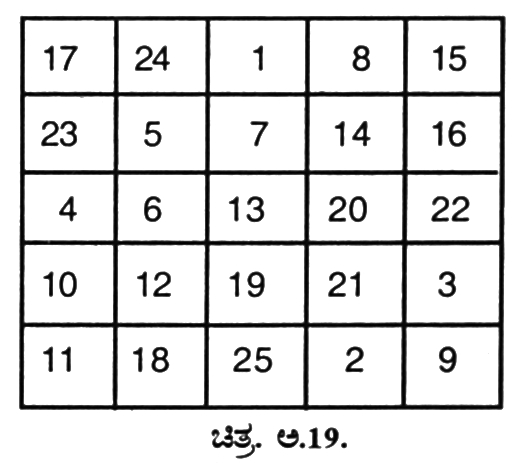
\includegraphics{src/figures/chap9/fig9-14.jpg}
\end{figure}

ಈ ವಿಧಾನದಲ್ಲಿ ಮಾಯಾಚೌಕ ರಚಿಸಿದಾಗ ಕೊನೆಯ ಸಂಖ್ಯೆ ಹೊರ ಆವರಣದ ಮನೆಯಲ್ಲಿ ಬರುತ್ತದೆ. ಅಲ್ಲಿಂದ ಒಂದು \textbf{‘ಭಂಗ ಚಲನೆ’} (Broken move) ಎಂದರೆ ಬಲಕ್ಕೆ ಮೇಲೇ\-ರಿ, ನಂತರ ಎಡಕ್ಕೆ ಮೇಲೇರಿದರೆ ಪ್ರಾರಂಭಿಕ ಸಂಖ್ಯೆ ದೊರೆಯುತ್ತದೆ. ಉದಾಹರಣೆಯಲ್ಲಿ 25 ಕೊನೆಯ ಸಂಖ್ಯೆಯಾಗಿದ್ದು ಕೆಳಗಿನ ಅಡ್ಡಸಾಲಿನ ಮಧ್ಯದ ಮನೆಯಲ್ಲಿದೆ. ಅಲ್ಲಿಂದ 2 ಮನೆ ಓರೆಯಾಗಿ 21,22 ರ ಮೂಲಕ ಮೇಲೇರಿ ಮತ್ತೆ 14ರ ಮೂಲಕ ಎಡಕ್ಕೆ ಮೇಲೇರಿದರೆ ಪ್ರಾರಂಭಿಕ ಸಂಖ್ಯೆ 1 ಸಿಕ್ಕುತ್ತದೆ. ಮತ್ತೆ ಮೊದಲಿನಂತೆ ಚೌಕವನ್ನು ಇನ್ನೊಂದು ಸುತ್ತು ಕ್ರಮಾಗತ ಸಂಖ್ಯೆಗಳ ಮೂಲಕ ಕ್ರಮಿಸಬಹುದು. ಇದೊಂದು ಅಂತ್ಯವಿಲ್ಲದ ಚಕ್ರ. ಹಿಂದೂ ನಂಬಿಕೆ\-ಯಾದ \textbf{‘‘ಪುನರಪಿ ಜನನಂ ಪುನರಪಿ ಮರಣಂ’’}ಗೆ ಇದನ್ನು ಸಮನ್ವಯಿಸಿದ್ದೂ ಉಂಟು. ಈ ವಿಧಾನವನ್ನು ಯೂರೋಪಿಗೆ ಪರಿಚಯಿಸಿದ್ದು \textbf{ಸೈಮನ್ ಡಿ ಲಾ ಲೌಬೋರೆ} ಎಂಬುವನು. \linebreak ಅವನು ಇದನ್ನು \textbf{‘‘ಹಿಂದೂ ವಿಧಾನ’’} ಎಂದು ಕರೆದಿದ್ದಾರೆ.

ಭಾರತದ ಜೈನ ಗಣಿತಜ್ಞರೂ ಸಹ ಮಾಯಾಚೌಕ ಕ್ಷೇತ್ರದಲ್ಲಿ ಕೈಯಾಡಿಸಿದ್ದುಂಟು. ಮಾನ\-ದೇವ ಸೂರಿ ಎಂಬಾತನು ತನ್ನ \textbf{‘ಲಘು ಶಾಂತಿ ಸ್ತೋತ್ರ’} ದಲ್ಲಿ 16 ಮನೆಗಳ ಮಾಯಾಚೌಕ ರಚಿಸಿ ಅದನ್ನು ಬೀಜಮಂತ್ರವಾಗಿ ಬಳಸುವುದನ್ನು ಸೂಚಿಸಿರುವನು. (ವಿವರಗಳಿಗೆ ಪುಟ 49 \linebreak ನೋಡಿ)

ಶುಭಸುಂದರ ಎಂಬಾತನು ತನ್ನ \textbf{‘‘ಯುಗಾದಿ ದೇವ ಸ್ತೋತ್ರದಲ್ಲಿ’’} 25 ಮನೆಗಳ ಮತ್ತು 64 ಮನೆಗಳ ಮಾಯಾಚೌಕಗಳನ್ನು ಕೊಟ್ಟಿದ್ದಾನೆ. ಧರ್ಮಾನಂದನೆಂಬುವನು 64 ಮನೆಗಳ ಮಾಯಾಚೌಕ ರಚಿಸುವ ಬೇರೊಂದು ವಿಧಾನವನ್ನು ತನ್ನ ಸ್ತೋತ್ರವೊಂದರಲ್ಲಿ ಕೊಟ್ಟಿರುವನು. ಇದರಿಂದ ಭಾರತದಲ್ಲಿ ಮಾಯಾಚೌಕಗಳ ಅಧ್ಯಯನ ಬಹಳ ಹಿಂದಿನ ಕಾಲದಿಂದ ನಡೆದಿರುವುದು ವೇದ್ಯವಾಗುತ್ತದೆ.

\section*{ಪಾಶ್ಚಾತ್ಯ ಜಗತ್ತು :}

ಬೈಜಾಂಟೈನ್ ವಿದ್ವಾಂಸ ಮಾನ್ಯುಯಲ್ ಮಾಸ್ಕೋಪೌಲಸ್ ಎಂಬುವನು ಕ್ರಿ.ಶ. 14ನೆ ಶತಮಾನದಲ್ಲಿ ತನ್ನ ಸ್ನೇಹಿತನಿಗೆ ಗ್ರೀಕ್ ಭಾಷೆಯಲ್ಲಿ ಬರೆದ ಪತ್ರವೊಂದರಲ್ಲಿ 3 ರಿಂದ 9 ರವರೆಗಿನ ಬೆಸಸಂಖ್ಯೆ ಕ್ರಮವರ್ಗದ ಮಾಯಾಚೌಕಗಳನ್ನು ರಚಿಸುವ ಬಗ್ಗೆ ವಿವರಿಸಿದ್ದಾರೆ. ಇದರಲ್ಲಿ ಚದುರಂಗದ ಕುದುರೆ ನಡಿಗೆಯಲ್ಲಿ ಸಂಖ್ಯೆಗಳನ್ನು ತುಂಬಿಸುವ ವಿಧಾನವೇ ಅಲ್ಲದೆ 4 ಮತ್ತು 8 ಕ್ರಮವರ್ಗಗಳ ಮಾಯಾಚೌಕಗಳ ರಚನೆ (ಇಸ್ಲಾಮಿಕ್ ವಿಧಾನ) ಯ ಉಲ್ಲೇಖವೂ ಲಭ್ಯವಿದೆ. ಮಾಸ್ಕೋ-ಪೌಲಸ್ನ ಕಾಲದ ನಂತರ ಈ ಪತ್ರವು ಬಯಲಿಗೆ ಬಂದಿತು. ಹಾಗಾಗಿ ಈ ಬಗೆಯ ಮಾಯಾಚೌಕ ರಚನೆಯ ಗೌರವ ಅವನಿಗೆ ಲಭಿಸಿತು. ಆದರೆ ವಾಸ್ತವವಾಗಿ ಮುಸ್ಲಿಂ ರಾಷ್ಟ್ರಗಳಲ್ಲಿ ಅಭಿವೃದ್ಧಿಗೊಂಡ ಈ ವಿಧಾನವನ್ನು ಅವನು ಸ್ಪೇನಿನ ಮೂಲಕ ಯೂರೋಪಿಗೆ ವರ್ಗಾಯಿಸಿದ್ದನು. ಸ್ಪೇನಿನಲ್ಲಿದ್ದ ಯಹೂದಿ ಮತ್ತು ಕ್ರಿಶ್ಚಿಯನ್ ವಿದ್ವಾಂಸರು ಮೂರ್ ಮತ್ತು ಅರಬ್ ಗಣಿತಜ್ಞರೊಂದಿಗೆ ಇವುಗಳ ಅಧ್ಯಯನ ನಡೆಸಿದರು. ಯಹೂದಿ ವಿದ್ವಾಂಸರಲ್ಲೊಬ್ಬನಾದ ಅಬ್ರಹಾಂ ಇಬ್ನ್ ಎಜ್ರಾ ಎಂಬುವನು ಟೊಲೆಡ್ ಪಟ್ಟಣದಲ್ಲಿ ಕ್ರಿ.ಶ. 17ನೆಯ ಶತಮಾನ\break ದಲ್ಲಿ 3 ಕ್ರಮವರ್ಗದ ಮಾಯಾಚೌಕವನ್ನು ಹೀಬ್ರೂ ಆಧ್ಯಾತ್ಮಿಕ ರಹಸ್ಯದೊಡನೆ ತಳುಕು ಹಾಕಿ ಪ್ರಕಟಿಸಿದನು. ಅವನ ತರುವಾಯದವರು ಅವನ ಹಾದಿಯಲ್ಲೇ ಮುಂದುವರೆದು ಮಾಯಾ ಚೌಕಗಳನ್ನು ಕಬಾಲಾ (ಯಹೂದೀ ಧರ್ಮತತ್ವಗಳು) ದೊಂದಿಗೆ ಹೊಂದಿಕೊಂಡ ಧಾರ್ಮಿಕ ಗಣಿತೀಯ ಊಹೆಗಳಾಗಿ ರೂಪಿಸಿದರು.

ಜರ್ಮನಿಯ ಹೈನರಿಕ್ ಕಾರ್ನೀಲಿಯಸ್ ಅಗ್ರಿಪ್ಪ ಫಾನ್ ನೆಟ್ಶೀಮ್​ ಮತ್ತು ಇಟಲಿಯ \hbox{ಗಿರೊಲಾಮೊ ಕಾರ್ಡಾನೊ} - ಇವರಿಬ್ಬರೂ 16ನೆಯ ಶತಮಾನದಲ್ಲಿ ಏಳು ಮಾಯಾಚೌಕಗಳ ಒಂದು ಗುಚ್ಛವನ್ನು ಸ್ವತಂತ್ರವಾಗಿ ರಚಿಸಿ, ಪ್ರಕಟಿಸಿದರು. ಈ ಚೌಕಗಳನ್ನು ಅಂದು ನಂಬಿಕೆಯಲ್ಲಿದ್ದ 

\medskip
ಸಪ್ತ ಗ್ರಹಗಳಿಗೆ (ಸೂರ್ಯ, ಚಂದ್ರ, ಕುಜ, ಬುಧ, ಶುಕ್ರ, ಗುರು ಮತ್ತು ಶನಿ) ಸಂಬಂಧಿಸಿ\-ದುವೆಂದು ಹೇಳಿದರು. ಬಹುಶಃ ಈ ಭಾವನೆ ಕಬಾಲಾ ಮೂಲದಿಂದ ಉಂಟಾಗಿರಬಹುದು. ಈ ಚೌಕಗಳು ಇಸ್ಲಾಮಿಕ್ ವಿಧಾನದಿಂದ ರಚಿತವಾಗಿದ್ದರೂ ಅವುಗಳ ನಿಜವಾದ ಮೂಲಗಳ ಪತ್ತೆಯಾಗಿಲ್ಲ. ಅಗ್ರಿಪ್ಪನು ರಚಿಸಿದ ಚೌಕಗಳು ಎರಡು ರೂಪಗಳಲ್ಲಿ ಅವನ \textbf{‘‘ಡಿ ಅಕ್ಕಲ್ಟ ಫಿಲಸಾಫಿಯ’’} ಗ್ರಂಥದಲ್ಲಿ (1531) ಹೊರಬಂದುವು. ಒಂದು ರೂಪ ಹೀಬ್ರೂ ಅಕ್ಷರ - ಸಂಖ್ಯೆಗಳನ್ನು ಬಳಸಿದರೆ ಮತ್ತೊಂದು ರೂಪ ಯೂರೋಪಿನಲ್ಲಿ ಬಳಕೆಯಲ್ಲಿದ್ದ ಹಿಂದೂ- ಅರಾಬಿಕ್ಸಂಖ್ಯೆಗಳನ್ನು ಬಳಸಿದ್ದಿತು. ಈ ಚೌಕಗಳನ್ನು ಲೋಹದ ಹಾಳೆಯ ಮೇಲೆ ಕೆತ್ತಿ, ತಾಯಿತವಾಗಿ ಬಳಸಿದರೆ ಶುಭವಾಗುವುದೆಂದು ಬರೆದಿದ್ದಾನೆ. ಅಷ್ಟೇ ಅಲ್ಲದೇ 1ನ್ನು ಒಳಗೊಂಡ ಒಂದು ಮನೆ ಚೌಕವು ಸೃಷ್ಟಿಕರ್ತನನ್ನು ಸೂಚಿಸುವುದಾಗಿ ಹೇಳಿದ್ದಾನೆ.

\medskip
ಅಗ್ರಿಪ್ಪನ ಸಮಕಾಲೀನನಾದ ಆಲ್ಬ್ರೆಕ್ಟ್ ಡ್ಯೂರರನು ಕ್ರಿ.ಶ. 1514ರಲ್ಲಿ 4 ಕ್ರಮವರ್ಗದ ಒಂದು ಸರಳ ಮಾಯಾಚೌಕವನ್ನು ತನ್ನ ಪ್ರಸಿದ್ಧ ಕೆತ್ತನೆ \textbf{‘‘ಮೆಲಂಕೊಲಿಯಾ 1’’} ರಲ್ಲಿ ರೂಪಿಸಿದನು. ಈ ಕೆತ್ತನೆಯು ಕಲೆ ಮತ್ತು ವಿಜ್ಞಾನ ವಿಷಯಗಳಲ್ಲಿ ಗಣಿತಶಾಸ್ತ್ರವನ್ನು ಪ್ರತಿನಿಧಿಸುವ \break ಚಿಹ್ನೆಯಾಗಿತ್ತು. ನಂತರದ ಬರಹಗಾರರು ಇದನ್ನು ಮಾಯಾಚೌಕಗಳ \hbox{ವ್ಯುತ್ಪತ್ತಿಯಲ್ಲಿ ಪ್ರಮಖ} ಕೊಂಡಿ ಎಂದು ಕೊಂಡಾಡಿದರು. (ಡ್ಯೂರರ್ ಚೌಕದ ವಿವರಗಳು ಪುಟ 52ರಲ್ಲಿವೆ) ವಾಸ್ತವ\-ವಾಗಿ ಈ ಚೌಕವು ಭಾರತ ಮತ್ತು ಮಧ್ಯಪ್ರಾಚ್ಯಗಳಲ್ಲಿ ಶತಮಾನಗಳ ಪೂರ್ವದಲ್ಲಿಯೇ ಬಳಸ\-ಲ್ಪಟ್ಟಿತ್ತು. ಸಂಪರ್ಕ ಮಾಧ್ಯಮಗಳು ಸೀಮಿತವಾಗಿದ್ದ ಆ ದಿನಗಳಲ್ಲಿ ಡ್ಯೂರರ್ನ ಚೌಕವು \linebreak ಯೂರೋಪಿನ ಸುಶಿಕ್ಷಿತರ ಗಮನವನ್ನು ಮಾಯಾಚೌಕಗಳ ಕಡೆಗೆ ಸೆಳೆಯುವುದರಲ್ಲಿ ಯಶಸ್ವಿ\-ಯಾಯಿತು.

\medskip
ಹಲವು ವರ್ಷಗಳ ನಂತರ ಜರ್ಮನಿಯ ಇಬ್ಬರು ವಿದ್ವಾಂಸರು ಮಾಯಾಚೌಕಗಳನ್ನು \hbox{ಶುದ್ಧ ಗಣಿತೀಯ} ದೃಷ್ಟಿಯಿಂದ ಅಧ್ಯಯಿಸಿದರು. ಕ್ರಿ.ಶ. 1544ರಲ್ಲಿ ಮೈಕೇಲ್ ಸ್ಟಿಫೆಲ್ನು ಆವರಣ ಮಾಯಾಚೌಕಗಳನ್ನು ರಚಿಸುವ ಹಳೆಯ ಇಸ್ಲಾಮಿಕ್ ವಿಧಾನಕ್ಕೆ ವಿವರಣೆ ಕೊಟ್ಟನು. ಆದರೆ ಇವನು ಬಳಸಿದ ರೀತಿ ಕಠಿಣವೆನಿಸಿದ್ದರಿಂದ ಯೂರೋಪಿನಲ್ಲಿ ಜನಪ್ರಿಯತೆಯನ್ನು ಗಳಿಸ\-ಲಿಲ್ಲ. ಇದಾದ ನಂತರ ಕ್ರಿ.ಶ.1550ರಲ್ಲಿ ಆಡಂ ರೀಸ್ ಎಂಬುವನು \hbox{ಮಾಯಾಚೌಕಗಳ ಕುರಿತ} ಪುಸ್ತಕಗಳ ಮಾಲೆಯನ್ನೇ ಹೊರತಂದನು. ಇವನ ಪುಸ್ತಕಗಳಲ್ಲಿ ಬೆಸಸಂಖ್ಯೆ ಕ್ರಮವರ್ಗದ ಮಾಯಾ\-ಚೌಕಗಳನ್ನು ಪರ್ಷಿಯನ್ ಸಾತತ್ಯ ವಿಧಾನ (Continous Method) ದಿಂದ ರಚಿಸು\-ವುದನ್ನು ಸರಳವಾಗಿ ವಿವರಿಸಿದ್ದಾನೆ. ಜೊತೆಗೆ ಸಮಸಂಖ್ಯೆ ಕ್ರಮವರ್ಗದ ಮಾಯಾಚೌಕ ಗಳಲ್ಲಿ ಸುಲಭ ವಾದವುಗಳನ್ನು ರಚಿಸುವ ರೀತಿಯನ್ನು ಕೊಟ್ಟಿದ್ದಾನೆ.

ಕ್ರಿ.ಶ. 17ನೆಯ ಶತಮಾನದ ಆದಿ ಭಾಗದಲ್ಲಿ ಕ್ರಿಶ್ಚಿಯನ್ ಕಾಬಾಲಿಸ್ಟರು (Cabalists) ಮಾಯಾಚೌಕಗಳಲ್ಲಿ ಆಸಕ್ತಿ ತಳೆದರು. ಇವರು ತಾವು ರಚಿಸಿದ ಚೌಕಗಳಲ್ಲಿ ಹೀಬ್ರೂ ಅಕ್ಷರ ಸಂಖ್ಯೆಗಳನ್ನು ಬಳಸಿದರು. ಯಹೂದಿಗಳು ತಾವು ರಚಿಸಿದ ಚೌಕಗಳಲ್ಲಿ 15ನ್ನು ‘‘ 9 ಮತ್ತು 6’’ ಎಂದು ಬರೆಯುತ್ತಿದ್ದರು. (15ನ್ನು ಬಳಸುತ್ತಿರಲಿಲ್ಲ)ಆದರೆ ಕ್ರಿಶ್ಚಿಯನ್ನ್ರು 15ನ್ನೇ ಬಳಸಿರುವುದು ಕಂಡುಬರುತ್ತದೆ. ಆ ಶತಮಾನದ ಕೊನೆಯ ವೇಳೆಗೆ \hbox{ಮಾಯಾಚೌಕಗಳ ಪ್ರಾಶಸ್ತ್ಯ } ಕುಂದಿತು. ಅವು ಕೇವಲ ಗಣಿತಾಧ್ಯಯನದಲ್ಲಿ ಮಾತ್ರ ಉಳಿದುಕೊಂಡವು. ಜರ್ಮನ್ನರು ಮಾಯಾಚೌಕಗಳಲ್ಲಿ ಸಾಧಿಸಿದ್ದ ವಿಷಯಗಳು ನೆರೆಯ ರಾಜ್ಯವಾದ ಫ್ರಾನ್ಸ್ಗೂ ತಲುಪಿದವು. \textbf{ಪಿಯರ್ ದ ಫರ್ಮಾ} (1601-65) \textbf{ಬಾಷೆ ದ ಮೆರಿಯಾಕ್} ಮತ್ತು \textbf{ಫಿಲಿಪ್ ದ ಲಾ ಹೈರ್} (1640-1718) ಮುಂತಾದವರು ಮಾಯಾಚೌಕಗಳನ್ನು ಸಂಖ್ಯಾ ವಿನ್ಯಾಸ ದೃಷ್ಟಿಯಿಂದ ಅಧ್ಯಯನ ಮಾಡಿದರು. ಮಾಯಾಚೌಕಗಳ ಬಗ್ಗೆ ವಿಶೇಷ ಅಧ್ಯಯನ ಮಾಡಿದ್ದ \textbf{ಬರ್ನಾರ್ಡ್ ಫ್ರೆನಿಕಲ್} (1602-1675) ಎಂಬುವನು ಅವುಗಳ ರಚನೆಯ ಕುರಿತಂತೆ ಬರೆದ ಏಕ ವಿಷಯ ಗ್ರಂಥವೊಂದು ಆ ಕಾಲದ ಶ್ರೇಷ್ಠ ಕೊಡುಗೆ ಎಂದು ಹೆಸರು ಮಾಡಿತು. ಈ ಗ್ರಂಥದ \hbox{ವೈಶಿಷ್ಟ್ಯ} ವೆಂದರೆ ಮೊದಲ ಬಾರಿಗೆ 4 ಕ್ರಮವರ್ಗದ ಎಲ್ಲ 880 ಬೇರೆ ಬೇರೆ ಚೌಕಗಳನ್ನು ಪ್ರಸ್ತುತ\break ಗೊಳಿಸಿದುದು.

18ನೆ ಶತಮಾನವು ಮಾಯಾಚೌಕಗಳ ಇತಿಹಾಸದಲ್ಲಿ ಸ್ಮರಣೀಯ. ಸ್ವಿಸ್ ಗಣಿತಜ್ಞ \linebreak \textbf{ಲಿಯೊನಾರ್ಡ್ ಆಯ್ಲರ್} (1707-1783) ಮತ್ತು ಅಮೇರಿಕೆಯ ಪ್ರತಿಭಾಶಾಲಿ \textbf{ಬೆಂಜಮಿನ್ ಫ್ರಾಂಕ್ಲಿನ್} (1706-1790) ಅನೇಕ ರೀತಿಯ ರಂಜನೀಯ ಮಾಯಾಚೌಕಗಳನ್ನು ರಚಿಸಿ ಜನ ಸಾಮಾನ್ಯರಿಗೆ ಸಂತಸ ತಂದುಕೊಟ್ಟರು. ದೈತ್ಯ ಪ್ರತಿಭೆಯ ಫ್ರಾಂಕ್ಲಿನ್ ಅಂತೂ ಹೊಸ ರೀತಿಯ ಮಾಯಾಚೌಕಗಳನ್ನೂ ರೂಪಿಸಿದನು. ಆ ಚೌಕಗಳಿಗೆ \textbf{‘‘ಫ್ರಾಂಕ್ಲಿನ್ ಚೌಕ’’} ಗಳೆಂದೇ ನಾಮ\-ಕರಣ ಮಾಡಲಾಗಿದೆ.

19 ಹಾಗೂ 20ನೆಯ ಶತಮಾನಗಳಲ್ಲಿ ಅಮೆರಿಕೆಯಲ್ಲಿ ಮಾಯಾಚೌಕಗಳ ಅಧ್ಯಯನ ಗಣನೀಯವಾಗಿ ಬೆಳೆಯಿತು. ಅದನ್ನು ಒಂದು ಬೌದ್ಧಿಕ ಕಾಲಕ್ಷೇಪವಾಗಿ ಗಣಿಸಲಾಯಿತು. ಹಿಂದೂ ಪದ್ಧತಿಯಿಂದ ಮಾಯಾಚೌಕ ರಚಿಸುವ ವಿಧಾನವನ್ನು ಅಭಿವೃದ್ಧಿಗೊಳಿಸಿ ಹೊಸ ರೀತಿಯ ಚೌಕಗಳನ್ನು ಸೃಷ್ಟಿಸಲಾಯಿತು. ಕೆಲವರಂತೂ 4 ಕ್ಕಿಂತ ಹೆಚ್ಚಿನ ಕ್ರಮವರ್ಗದ ಮಾಯಾಚೌಕಗಳಲ್ಲಿ ಪಡೆಯಬಹುದಾದ ಗರಿಷ್ಠ ಪರಿಮಾಣವನ್ನು ಲೆಕ್ಕಹಾಕುವ ಯತ್ನ ಮಾಡಿದರು. ಈ ಹಿಂದೆ ಯಾರೂ ಈ ದಿಶೆಯಲ್ಲಿ ಕೆಲಸ ಮಾಡಿರಲಿಲ್ಲ. ಮತ್ತೆ ಕೆಲವರು ಎಲ್ಲ ಮಾಯಾಚೌಕಗಳ ರಚನೆಗೆ ಅನ್ವಯಿಸಬಹುದಾದ ಒಂದೇ ಸೂತ್ರವನ್ನು ರೂಪಿಸುವಲ್ಲಿ ಶ್ರಮಿಸಿದರು. \hbox{ಇಷ್ಟಾದರೂ} 2000 ವರ್ಷಗಳ ಅಧ್ಯಯನ, ಪ್ರಯೋಗ, ಪರಿಶೀಲನೆಗಳ ನಂತರವೂ ಮಾಯಾಚೌಕಗಳ \linebreak ಕ್ಷೇತ್ರದಲ್ಲಿ ಸಾಧಿಸಬೇಕಾದುದು ಬಹಳಷ್ಟಿದೆ.
\begin{center}
*****
\end{center}
